%% Artículo del proyecto final -- Procesamiento de Lenguaje Natural (ISIS 4221)
%% Plantilla: ACM Conference Proceedings (acmart, formato sigconf)
\documentclass[sigconf,nonacm]{acmart}
\usepackage[T1]{fontenc}
\usepackage[english,spanish.noshorthands.tabla.nodecimaldot.notilde.noquoting]{babel}

\renewcommand\keywordsname{Palabras clave}
\usepackage{booktabs}
\usepackage{multirow}
\usepackage{amsmath}
\usepackage{newunicodechar}
\newunicodechar{−}{\ensuremath{-}}
\newunicodechar{±}{\ensuremath{\pm}}
\newunicodechar{×}{\ensuremath{\times}}
\newunicodechar{→}{\ensuremath{\rightarrow}}
\newunicodechar{↔}{\ensuremath{\leftrightarrow}}
\newunicodechar{≈}{\ensuremath{\approx}}
\newunicodechar{≤}{\ensuremath{\leq}}
\newunicodechar{λ}{\ensuremath{\lambda}}
\newunicodechar{α}{\ensuremath{\alpha}}
\newunicodechar{γ}{\ensuremath{\gamma}}
\newunicodechar{⁻}{\textsuperscript{\ensuremath{-}}}
\newunicodechar{⁴}{\textsuperscript{4}}

\AtBeginDocument{%
  \providecommand\BibTeX{{Bib\TeX}}%
  \renewcommand{\tablename}{Tabla}%
  \renewcommand{\listtablename}{Índice de tablas}}
\addto\captionsspanish{\renewcommand{\tablename}{Tabla}}

\begin{document}
\setlength{\parskip}{0pt plus 4pt}\allowdisplaybreaks

\title{Corrección y detección genética una aproximación desde el problema de la corrección ortográfica}

\author{Azul Jacob Manzano Piñeros}
\affiliation{%
  \institution{Universidad de los Andes}
  \city{Bogotá}
  \country{Colombia}}
\email{aj.manzano@uniandes.edu.co}

\author{Daniel Escalante Perez}
\affiliation{%
  \institution{Universidad de los Andes}
  \city{Bogotá}
  \country{Colombia}}
\email{d.escalante@uniandes.edu.co}

\author{Brenda Jimena Babativa Santos}
\affiliation{%
  \institution{Universidad de los Andes}
  \city{Bogotá}
  \country{Colombia}}
\email{b.babativa@uniandes.edu.co}

\begin{abstract}
La secuenciación de nueva generación es un conjunto de tecnologías que permiten determinar el orden de los nucleótidos de una secuencia genética, a pesar de su extendido uso, es una tecnología que sigue siendo propensa a errores, con tasas de error medianas entre 0.087 \% y 0.613 \% según la plataforma de Illumina, donde esta variabilidad va a depender en mayor medida del experimento que de la plataforma~\cite{stoler2021sequencing}. Los correctores existentes dependen de la redundancia de las lecturas~\cite{mitchell2020benchmarking} donde la mayor limitante va a estar mediada por la cobertura. En este trabajo abordamos la detección y corrección de sustituciones de nucleótidos en una única secuencia codificante, tratándola como un problema de corrección ortográfica. Proponemos entonces ajustar GENERanno-prokaryote-0.5b-base, un transformer bidireccional con tokenización nucleótido por nucleótido, mediante LoRA y una cabeza de clasificación por posición. Los errores se simulan sobre genes de E. coli con tasas de 0.1\%, 1\% y 5\% y con perfiles uniformes y realistas de Illumina, y el modelo se compara con 4 líneas base (sin cambios, corrector por frecuencia, n-gramas con canal ruidoso y GENERanno sin ajuste), con la ganancia como métrica principal y métricas de detección, corrección y sobrecorrección, con partición por gen y una prueba fuera de dominio con \emph{Haloferax volcanii.} El modelo ajustado obtuvo la mayor ganancia en \emph{E. coli} en todas las tasas, superó a los n-gramas con intervalos de confianza que excluyen el cero y redujo la sobrecorrección del modelo sin ajustar. Con detección perfecta eligió la base correcta en el 98.5 \% de los errores con el 1 \%. Los errores sinónimos fueron identificados en este trabajo como los más difíciles, o en términos de la analogía utilizada los errores ortográficos que producen otra palabra válida. Por otra parte, la ganancia depende de la tasa de error y el modelo no generalizó a la arquea utilizada.
\end{abstract}

\keywords{errores de secuenciación, LoRA, GENERanno, Illumina, Next generation sequencing, transformer}

\maketitle
\renewcommand{\shortauthors}{Manzano Piñeros, Escalante Perez y Babativa Santos}

\section{Introducción}\label{sec:introduccion}

La secuenciación de nueva generación (NGS) por sus siglas en inglés, son una serie de herramientas y tecnologías ampliamente usadas en investigación genética, y aunque las tecnologías de secuenciación se han ido mejorando desde las primeras como sanger, lo cierto es que siguen manteniendo tasas de error medianas entre el 0.087 \% y el 0.613 \% en plataformas de Illumina~\cite{stoler2021sequencing} a priori pueden parecer tasas bajas de error, sin embargo esto puede ser una limitante en su uso clínico en contextos puntuales pues por ejemplo los indels pueden ser de apenas un par de nucleótidos. Además el error no es uniforme de acuerdo con Stoler y Nekrutenko~\cite{stoler2021sequencing} donde para llegar a esta conclusión analizaron múltiples corridas de \emph{E. coli} en siete instrumentos de illumina y encontraron medianas entre 0.087\% y 0.613\% encontrando que existe una mayor variación entre corridas de una misma plataforma que entre diferentes plataformas. Por lo que la calidad es algo que no puede asumirse,

Los métodos computacionales de corrección más comunes se basan en k-mers y requieren ver cada región varias veces (Valiéndose de la cobertura) Mitchell et al.~\cite{mitchell2020benchmarking} evalúan diez correctores y concluyen que ningún método es superior en todos los tipos de datos, así mismo concluye que los mejores resultados se obtienen en coberturas superiores a 4x y que en poblaciones muy heterogéneas casi todos los métodos fallan.

En este trabajo adaptamos la analogía de la corrección ortográfica a la corrección de DNA, donde los nucleótidos son letras, los codones son palabras, y las secuencias son oraciones. El problema consiste en que dada una secuencia con posibles cambios o sustituciones, se intenta entonces determinar en qué posiciones hay un error (detección) y cual debería ser la base correcta en ese punto (corrección). Nuestro acercamiento consiste en aprendizaje por transferencia desde GENERanno, un transformer con atención bidireccional y tokenización por nucleótido preentrenado con ADN procariota, ajustado con LoRA y una cabeza de clasificación por posición, siguiendo la formulación de detectar y corregir sustituciones token por token de soft masked BERT~\cite{zhang2020spelling}. Las contribuciones de este trabajo son:
\begin{itemize}
  \item La formulación de la corrección de errores de secuenciación como etiquetado por nucleótido sobre una sola secuencia, sin depender de la redundancia, ajustando GENERanno con LoRA y una cabeza de clasificación por posición.
  \item Una simulación de errores de sustitución con tasas de 0.1 \%, 1 \% y 5 \% y con perfiles uniformes y realistas de Illumina.
  \item Una evaluación que separa la detección de la corrección, que incluye la evaluación con oráculo y el análisis a nivel de gen, de codón y por categorías.
  \item La comparación con cuatro líneas base (sin cambios, corrector por frecuencia, N-gramas con canal ruidoso y GENERanno sin ajuste) y una prueba fuera de dominio con \emph{H. volcanii}.
\end{itemize}

\section{Trabajo relacionado}\label{sec:trabajo-relacionado}

\subsection{\texorpdfstring{Errores de secuenciación (Stoler y Nekrutenko)~\cite{stoler2021sequencing}}{Errores de secuenciación (Stoler y Nekrutenko)}}

En este trabajo se mide el error de illumina aprovechando las regiones donde se solapan los dos extremos de una lectura pareada, lo que atribuye las diferencias al instrumento y no a la preparación de la librería. Encontraron que los errores tienden a repetir la base anterior, que ciertos trímeros como GGT están sobrerrepresentados y que el error crece hacia al extremo 3'

Sus hallazgos son los que más condicionan nuestro diseño. Las medianas de error van de 0.087 \% (HiSeq X Ten) a 0.613 \% (MiniSeq), pero la variación entre corridas de una misma plataforma es mayor que entre plataformas (hasta 0.94 puntos porcentuales de desviación en MiSeq).

Incluimos este trabajo porque demuestra que el problema es real y variable, por lo que no se puede asumir la calidad de datos ajenos. Además, justifica las tasas de error que simulamos (0.1 \%, 1 \% y 5 \%). Siendo en adición la base de nuestro perfil realista: el error creciente por lectura y el sesgo posterior a homopolímeros de la Sección~\ref{sec:simulacion} salen directamente de este artículo. También lo leímos con cautela: asume que lo observado en E. coli se generaliza a otros organismos y su análisis favorece las corridas con mayor solapamiento, de modo que las muestras no son aleatorias.

\subsection{\texorpdfstring{Correctores basados en redundancia (Mitchell et al.)~\cite{mitchell2020benchmarking}}{Correctores basados en redundancia (Mitchell et al.)}}

En este trabajo se compararon diez correctores, casi todos basados en k-mers y mostraron que su desempeño depende de la cobertura y de la heterogeneidad de la muestra. Además, su evaluación requiere alinear secuencias por la presencia de recortes e indels, y no separa la detección de la corrección.

Lo incluimos porque es el mapa de lo que se ha hecho en corrección computacional y porque define con claridad qué limitación queremos evitar: la dependencia de la redundancia. De este trabajo tomamos la métrica principal, la ganancia, y la evaluación por base. Además, nos permite señalar dos diferencias concretas. Al limitarnos a sustituciones, las secuencias de entrada, con errores y corregida tienen la misma longitud, así que comparamos posición por posición sin alinear. Y como ellos no separan la detección de la corrección, nosotros las evaluamos por separado, incluyendo la evaluación con oráculo

\subsection{Transformers y modelos de lenguaje para secuencias}

\textbf{DeepConsensus} ~\cite{baid2021deepconsensus} Baid et al. corrigen lecturas PacBio HiFi con un transformer de solo encoder (6 capas, dimensión oculta de 560 y 2 cabezas de atención), entrenado desde cero. El modelo recibe ventanas de 100 bases con el alineamiento de hasta 20 subreads, el consenso de la herramienta estándar (pbccs) y señales del secuenciador, y predice por posición una distribución sobre A, C, G, T y un símbolo de hueco. Dado que la mayoría de los errores son inserciones y deleciones, proponen una pérdida basada en alineamiento calculada con programación dinámica diferenciable. Con ella reducen 41.9 \% los errores por lectura (de 24.61 a 14.31), y validan con cromosomas no vistos y con cuatro individuos distintos al de entrenamiento.

Lo incluimos porque es la referencia de corrección de errores de secuenciación con transformers y muestra que una arquitectura de atención que predice un símbolo por posición puede superar a un método estadístico establecido. También nos sirve de contraste: DeepConsensus corrige comparando hasta 20 copias de la misma molécula, mientras que nuestro modelo trabaja con una sola secuencia. Entrena desde cero con 128 núcleos TPU v3, mientras que nosotros ajustamos un modelo preentrenado con una sola GPU. Por último, justifica nuestra decisión de excluir inserciones y deleciones, que a ellos los obligaron a diseñar una pérdida especial; al limitarnos a sustituciones podemos usar entropía cruzada estándar. De allí tomamos también la idea de separar entrenamiento y prueba por unidades biológicas completas (ellos por cromosoma, nosotros por gen).

\textbf{Athena} ~\cite{abdallah2019athena} Abdallah et al.abordan un problema distinto al de corregir: ayudar a configurar los correctores existentes. Herramientas como Lighter, Blue y RACER, diseñadas para lecturas cortas de Illumina, dependen de un parámetro elegido por el usuario, normalmente la longitud \emph{k} de los k-mers, cuyo mejor valor cambia según los datos y que se encuentra alineando cada resultado contra un genoma de referencia, lo cual es lento e imposible si no hay referencia. Para evitarlo, Athena entrena un modelo de lenguaje con las lecturas sin corregir (un trigrama sobre «palabras» de 7 nucleótidos con SRILM, o una red recurrente a nivel de carácter con 2 capas de 300 neuronas). Luego una submuestra de lecturas se corrige con la herramienta externa usando distintos valores de \emph{k}, y se calcula la perplejidad de cada resultado. Como la perplejidad baja cuando la corrección es mejor, Athena elige el \emph{k} que la minimiza mediante hill climbing. La correlación entre perplejidad y calidad de corrección va de −0.93 a −0.98 en seis de siete conjuntos. Es importante aclarar que Athena no corrige ni localiza errores: las correcciones las hacen los correctores externos, y el modelo de lenguaje solo califica su trabajo.

Lo incluimos porque es uno de los primeros trabajos que aplica explícitamente modelos de lenguaje de NLP a los errores de secuenciación, y muestra de forma empírica que un modelo entrenado solo con ADN «nota» cuando una secuencia tiene errores (las sustituciones elevan la perplejidad hasta 4.7 veces más que las deleciones). Esa es la premisa de todo nuestro proyecto. Además, dos de sus conjuntos de datos son de \emph{E. coli} K-12, el mismo organismo que usamos. De él tomamos tres cosas: la configuración de n-gramas que inspiró nuestra línea base, la elección de una red a nivel de carácter para no tener que segmentar el ADN en «palabras», y el dato de que en Illumina las sustituciones son cerca del 99 \% de los errores. También aprendimos de su simulación: al sustituir eligen la nueva base al azar entre las cuatro, por lo que una de cada cuatro «sustituciones» deja la base igual y contamina las etiquetas; en nuestra simulación la base nueva siempre es distinta. La diferencia de fondo es que su modelo califica el trabajo de otros correctores, mientras que el nuestro detecta y corrige posición por posición.

\textbf{VESTIGE} ~\cite{chakravertty2026vestige} Chakravertty y Maheshwari ajustan DNABERT-2 (117 millones de parámetros, tokenización BPE) con una estrategia de enmascaramiento sensible al daño (DAM). En lugar de enmascarar el 15 \% de los tokens al azar, enmascaran citosinas y guaninas con probabilidad proporcional al daño medido por posición con mapDamage2, y reescalan las probabilidades para que el promedio siga siendo del 15 \%. Con el enmascaramiento estándar el modelo queda por debajo de un predictor aleatorio en las posiciones más cercanas a los extremos, mientras que con DAM lo supera por entre 4 y 10 puntos porcentuales.

Es el trabajo publicado más cercano al nuestro: ajusta un modelo de lenguaje genómico preentrenado para recuperar bases corrompidas, a partir de secuencias limpias con corrupción simulada, que es exactamente nuestro esquema experimental. Respalda el que simulemos perfiles de error realistas, mantener el promedio de error al hacerlo (reescalamos la distribución igual que ellos) y usar tokenización por nucleótido, porque con BPE dos sustituciones llegaron a alterar 31 tokens. Su método difiere del nuestro en que el error es de otro tipo (daño postmortem), en otro organismo, y en que las posiciones dañadas se reemplazan por {[}MASK{]}, de modo que el modelo solo adivina la base y no tiene que encontrar el error.

\subsection{\texorpdfstring{Modelos genómicos fundacionales (GENERanno)~\cite{li2025generanno}}{Modelos genómicos fundacionales (GENERanno)}}

Li et al. proponen un transformer con la arquitectura de Llama modificada para usar atención bidireccional en todas sus capas. Tiene cerca de 500 millones de parámetros, dimensión oculta de 1280, 16 cabezas de atención y un contexto de 8192 tokens, con tokenización por nucleótido. Se preentrenó con modelado de lenguaje enmascarado sobre 715 mil millones de nucleótidos de regiones funcionales de procariotas de RefSeq: se selecciona el 15 \% de los tokens, de los cuales el 80 \% se reemplaza por una máscara, el 10 \% por un nucleótido aleatorio y el 10 \% se deja igual. Lo ajustaron con cabezas de clasificación por token para anotar genes y evaluaron una colección de tareas propias, además de un genoma de arqueas no visto durante el preentrenamiento.

Es el modelo que ajustamos, y lo elegimos por razones específicas. La tokenización por nucleótido hace que cada sustitución afecte un solo token y evita decidir cómo segmentar el ADN. La atención bidireccional permite usar el contexto a ambos lados, que es lo que hace falta para decidir si una base encaja. El 10 \% de reemplazo aleatorio durante el preentrenamiento se parece a la sustitución que queremos corregir. El contexto de 8192 tokens cubre el gen más largo de nuestros datos, y los autores ya lo ajustaron con una cabeza por nucleótido, que es la estructura que requiere nuestra tarea. También es viable con recursos modestos (nosotros usamos una sola GPU). Su principal consideración para nuestro trabajo es que, según sus autores, no incluyó arqueas, lo que nos permite usarlas como prueba fuera de dominio, y que sí pudo incluir \emph{E. coli}, lo que declaramos como limitación.

\subsection{\texorpdfstring{Corrección ortográfica: Soft-Masked BERT~\cite{zhang2020spelling}}{Corrección ortográfica: Soft-Masked BERT}}

corrige errores ortográficos del chino a nivel de carácter con una red de detección y una de corrección basada en BERT, entrenadas con errores artificiales en texto correcto. Los autores señalan que BERT ajustado tiende a copiar la entrada en lugar de corregir, riesgo que abordamos con la pérdida ponderada y con la línea base sin cambios

Es el análogo en lenguaje natural de nuestro problema y la razón por la que formulamos la tarea como lo hacemos: sustituciones únicamente, entrada y salida de igual longitud, un token por carácter, y entrenamiento con errores artificiales sobre texto correcto. De este trabajo tomamos tres ideas. La primera es el riesgo de que BERT ajustado copie la entrada en lugar de corregir, que motivó nuestra línea base sin cambios y la pérdida ponderada. La segunda es la evaluación restringida a las posiciones con error, que estima el límite superior si la detección fuera perfecta y que adaptamos en la Sección~\ref{sec:oraculo}. La tercera es reportar tanto métricas por posición como por unidad completa, que nosotros hacemos con el porcentaje de genes perfectos. Lo que cambia es el alfabeto: ellos trabajan con miles de caracteres y nosotros con cuatro nucleótidos, así que la distribución de errores plausibles es muy distinta.

\section{Datos}\label{sec:datos}

\subsection{Descripción, estadísticas y preprocesamiento}\label{sec:datos-descripcion}

Los datos utilizados vienen de RefSeq, del National Center for Biotechnology Information (NCBI). El conjunto principal son las secuencias codificantes del genoma de referencia de \emph{Escherichia coli} K-12 substr. MG1655 (ASM584v2, GCF\_000005845.2)~\cite{ncbi_ecoli}, usado para entrenamiento, validación y prueba. Como prueba por fuera del dominio se usan las secuencias codificantes de la archea \emph{Haloferax volcanii} DS2 (ASM2568v1, GCF\_000025685.1)~\cite{ncbi_hvolcanii}, siendo necesario mencionar que estas nunca se usan para entrenar, esto basado en lo que los autores describen, GENERanno no se preentrenó con arqueas~\cite{li2025generanno}, por lo que este conjunto de datos nos permite verificar si el modelo aprendió patrones generales del ADN y no solo lo visto en el pre entrenamiento. Los datos son públicos; el NCBI no impone restricciones a su uso~\cite{ncbi_policies}, aunque advierte que los depositantes originales podrían reclamar derechos sobre parte de la información.

Los archivos están en formato FASTA (.fna)~\cite{ncbi_fasta} y cada entrada, con encabezado y secuencia, corresponde a una secuencia codificante. \emph{E. coli} contiene 4,318 secuencias con más de 4 millones de nucleótidos, y \emph{H. volcanii} 4,017 secuencias con más de 3.4 millones. Se descartaron las secuencias no aptas, aplicando los filtros (cada secuencia se cuenta en el primer criterio que la descarta): pseudogenes, secuencias parciales, excepciones de traducción, caracteres fuera de ACGT, longitud no múltiplo de 3, codones de inicio o de fin inválidos y duplicados. Tras el filtrado quedan 4,255 genes de \emph{E. coli} y 3,873 de arqueas.

La Tabla~\ref{tab:datos} resume las estadísticas de ambos conjuntos antes y después del filtrado, junto con la partición utilizada.

\begin{table}[t]
\caption{Estadísticas de los conjuntos de datos antes y después del filtrado}
\label{tab:datos}
\footnotesize
\setlength{\tabcolsep}{4pt}
\begin{tabular}{@{}lrr@{}}
\toprule
\textbf{Estadística} & \textbf{\emph{E. coli}} & \textbf{\emph{H. volcanii}} \\
\midrule
Secuencias codificantes en el archivo & 4,318 & 4,017 \\
Nucleótidos en el archivo & 4,026,887 & 3,465,867 \\
\midrule
Descartadas: pseudogenes & 18 & 120 \\
Descartadas: excepciones de traducción & 6 & 2 \\
Descartadas: secuencias duplicadas & 39 & 22 \\
Descartadas: demás filtros & 0 & 0 \\
\midrule
Genes tras el filtrado & 4,255 & 3,873 \\
Longitud media (nt) & 932.0 & 866.9 \\
Contenido de GC & 51.9 \% & 66.6 \% \\
GC en la tercera posición del codón & 56.0 \% & 86.1 \% \\
GC por gen del 90 \% de los genes & 40--57 \% & 56--73 \% \\
Codón más frecuente & CTG & GAC \\
Genes con codón de inicio ATG & 90.2 \% & 86.0 \% \\
Codón de parada más común & TAA (64.0 \%) & TGA (59.6 \%) \\
\midrule
Entrenamiento / validación / prueba & 3,407 / 415 / 433 & -- / -- / 3,873 \\
\bottomrule
\end{tabular}

\vspace{2pt}\parbox{\columnwidth}{\footnotesize Cada gen se cuenta en el primer filtro que lo descarta; los filtros de CDS parcial, caracteres fuera de ACGT, longitud no múltiplo de 3 y codones de inicio o de parada inválidos no descartaron genes adicionales. Desde «Genes tras el filtrado», los valores se calculan sobre los genes limpios; el gen más largo de los dos conjuntos tiene 7,020 nt, por debajo del contexto de 8,192 tokens del modelo. La partición de \emph{E. coli} se hizo por grupos de proteínas similares (MMseqs2, 50 \% de identidad y 80 \% de cobertura), para que genes casi idénticos no queden a la vez en entrenamiento y en prueba; los genes de \emph{H. volcanii} solo se usan como prueba.}
\end{table}

Estos datos son adecuados para el problema por tres razones. Primero, son secuencias codificantes completas y curadas (sin pseudogenes, secuencias parciales ni duplicados), por lo que la base correcta en cada posición es conocida con certeza; esto permite inyectar errores de sustitución con tasa y perfil controlados y evaluar detección y corrección posición por posición, algo que con lecturas reales solo se conoce de forma indirecta. Además, al no tener intrones, se evita la ambigüedad entre región codificante y región genómica~\cite{chakravertty2026vestige}, y su estructura de codones (inicio, interior y parada) sostiene la analogía con oraciones, palabras y letras. Segundo, son compatibles con el modelo: están en nucleótidos puros, como exige la tokenización por nucleótido de GENERanno, y ninguna secuencia supera los 8,000 nucleótidos, por debajo de su ventana de 8,192 tokens, así que cada gen entra completo sin fragmentarse. Tercero, permiten separar lo aprendido de lo preentrenado: \emph{E. coli} pertenece al dominio con el que se preentrenó el modelo, por lo que este ya tiene conocimiento previo que solo hay que especializar, aunque pudo haber visto este genoma; para controlarlo se usa \emph{H. volcanii}, un dominio genuinamente distinto,con un contenido de GC de 66.6 \% frente a 51.9 \% en E. coli (86.1 \% frente a 56.0 \% en la tercera posición del codón) y codones predominantes diferentes (el más frecuente es CTG en E. coli y GAC en H. volcanii, y el codón de parada más común es TAA en E. coli y TGA en H. volcanii). La contrapartida es que los errores se simulan sobre secuencias de referencia y no provienen de lecturas reales, y que se usa un solo organismo para entrenar y uno para la prueba fuera de dominio, limitaciones que se retoman en la Sección~\ref{sec:limitaciones}.

La Fig.~\ref{fig:gc} muestra el contenido de GC frente a la longitud de cada gen en ambos organismos: el 90 \% de los genes de \emph{E. coli} tiene entre 40 \% y 57 \% de GC, y el de \emph{H. volcanii}, entre 56 \% y 73 \%, por lo que los dos organismos casi no se solapan en composición.

\begin{figure*}[t]
  \centering
  \begin{minipage}{0.49\textwidth}\centering
    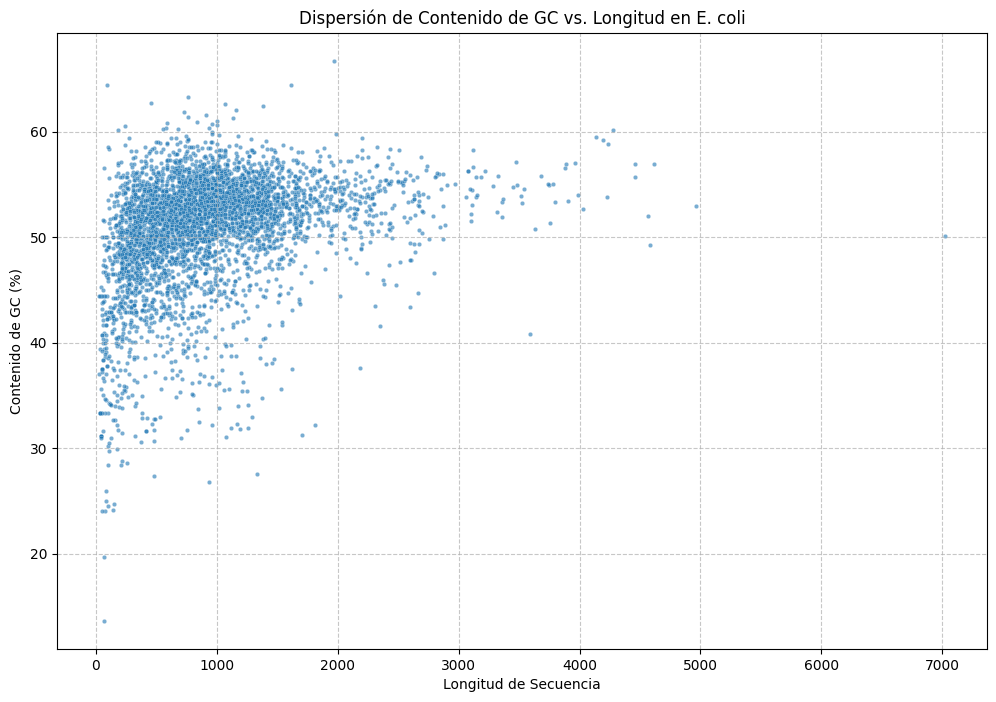
\includegraphics[width=\linewidth]{figuras/fig_dispersion_gc_ecoli.png}\\(a) \emph{E. coli}
  \end{minipage}\hfill
  \begin{minipage}{0.49\textwidth}\centering
    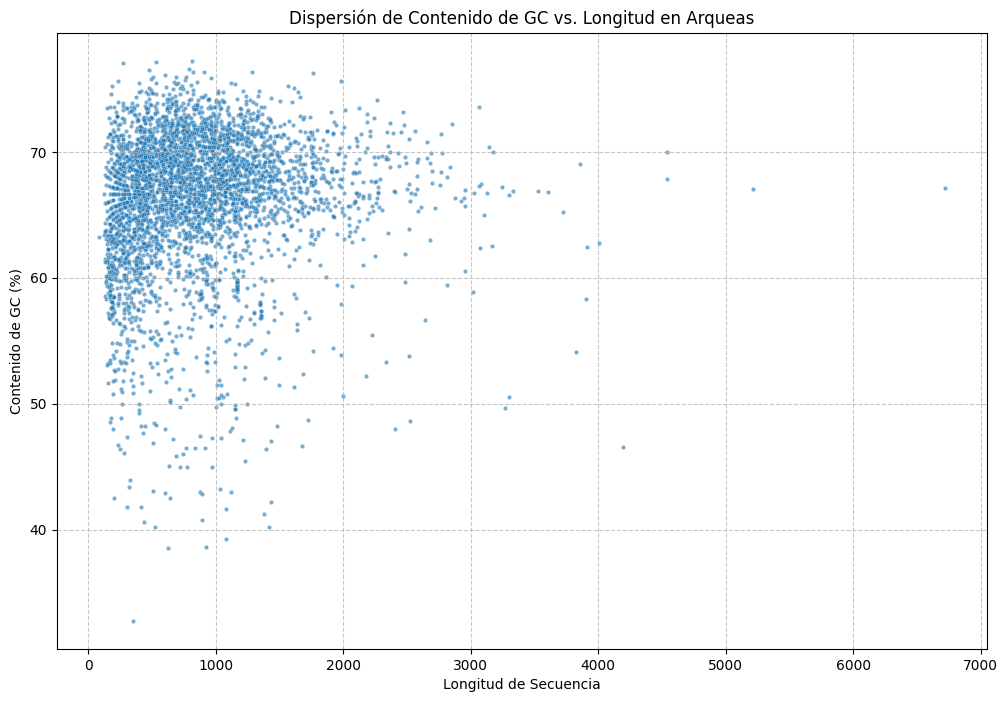
\includegraphics[width=\linewidth]{figuras/fig_dispersion_gc_hvolcanii.png}\\(b) \emph{H. volcanii}
  \end{minipage}
  \caption{Contenido de GC frente a la longitud de cada gen limpio en \emph{E. coli} (a) y \emph{H. volcanii} (b).}
  \Description{Dos diagramas de dispersión del contenido de GC frente a la longitud de cada gen: los genes de E. coli se concentran alrededor de 50 por ciento de GC y los de H. volcanii alrededor de 65 por ciento.}
  \label{fig:gc}
\end{figure*}

\subsection{Simulación de errores}\label{sec:simulacion}

Para la simulación de errores sobre las secuencias limpias se decidió tratar solamente errores de tipo sustitución a nivel de nucleótido. La primera razón para hacer esto es que, según lo que mencionan Abdallah et al. en~\cite{abdallah2019athena}, en los datos de Illumina se observa que los errores de sustitución conforman cerca del 99 \% de los errores. No obstante, diferimos de este otro estudio en que reemplazamos solamente con bases diferentes a la real: en ese estudio la nueva base se elige al azar entre las cuatro, por lo que una de cada cuatro sustituciones deja la base igual, lo que contaminaría las etiquetas.

Se decidió utilizar la tokenización y la simulación de errores a nivel de nucleótido ya que, de esta forma, el problema se puede definir como una clasificación de muchas entradas a muchas salidas. Este nivel de granularidad también ahorra el esfuerzo que habría que hacer para realinear las secuencias de origen, destino y etiquetas si se llegaran a tener inserciones o deleciones, como tuvieron que hacer Mitchell et al. en~\cite{mitchell2020benchmarking} y Baid et al. en~\cite{baid2021deepconsensus}. Esta decisión es apoyada por Zhang et al. en~\cite{zhang2020spelling} y Abdallah et al. en~\cite{abdallah2019athena}, ya que de esta forma no hay que definir cómo segmentar las palabras compuestas de nucleótidos, que, con un tokenizador, podrían causar distintas fronteras y tamaños de palabras dependiendo del contenido y del error insertado, como explican Chakravertty y Maheshwari en~\cite{chakravertty2026vestige}. Adicionalmente, usar solo sustituciones a nivel de nucleótido permite mantener la misma longitud para las entradas y las etiquetas.

Para la creación de las secuencias con ruido, se introdujo otra variable importante para estudiar, la cual era la probabilidad de error en cada posición. Dentro del proyecto se exploraron las siguientes tasas: 0.1 \%, 1 \% y 5 \%. Se estudiaron estos valores ya que, como se menciona en~\cite{stoler2021sequencing}, en distintas plataformas de Illumina se encontraron medianas de la tasa de error desde 0.087 \% (HiSeq X Ten) hasta 0.613 \% (MiniSeq). Adicionalmente, Illumina especifica para sus equipos NextSeq 1000 y 2000, con la química XLEAP-SBS, que entre el 85 \% y el 90 \% de las bases, según la longitud de lectura, tienen una calidad Q30 o superior, es decir, una probabilidad de error de 0.1 \% o menos~\cite{illumina_nextseq}. Por estas referencias, se eligieron esos valores para las primeras dos tasas. Como caso de estrés, se eligió usar 5 \% ya que, como se menciona en~\cite{abdallah2019athena}, existen conjuntos de datos reales con tasas de error de hasta el 43 \%.

Otro aspecto que se decidió incluir en la simulación de errores fue la utilización de un perfil de probabilidad uniforme en todos los nucleótidos de una secuencia, y de un perfil realista, que se asemeja a cómo se producen los errores en la realidad. Tomar esta decisión y evaluar los modelos sobre datos en diferentes modalidades es importante ya que, como mencionan Stoler y Nekrutenko~\cite{stoler2021sequencing}, los errores no suelen ser uniformes. Más específicamente, mencionan que en las tecnologías de Illumina los errores tienden a repetir la base anterior y que el error crece hacia el extremo 3\textquotesingle{} de la lectura. El uso de ambos perfiles también es respaldado por Chakravertty y Maheshwari en~\cite{chakravertty2026vestige}, quienes comparan una corrupción uniforme con una basada en el perfil de daño real y muestran que entrenar solo con corrupción uniforme, cuando la real no lo es, puede hacer que un modelo sea peor que el azar en ciertas posiciones clave.

Para configurar el perfil realista se tomaron varias decisiones. Primero que todo, las probabilidades realistas de error se calculan por lectura y no por gen; por lo tanto, al determinar las probabilidades, el gen se segmenta en grupos de 150 nucleótidos, ya que esta es una longitud de lectura estándar en Illumina. Esta decisión se toma ya que en varias fuentes, como Stoler y Nekrutenko~\cite{stoler2021sequencing}, se especifica que el error aumenta hacia el final de la lectura, y no hacia el final del gen. Entonces, se definió una pendiente que fuera incrementando la probabilidad de error desde el inicio de la lectura hasta el final de esta; en nuestro caso, elegimos una pendiente de 3 sobre la longitud total de la lectura, para que la última posición tuviera 4 veces la probabilidad de la primera.

Otro aspecto importante incluido en el perfil realista son los sesgos de contexto que mencionan Stoler y Nekrutenko~\cite{stoler2021sequencing}. Para nuestro proyecto implementamos el sesgo post-homopolímero, el cual incrementa la probabilidad de error después de una racha de nucleótidos repetidos. Se implementó que, luego de una racha de 3 o más nucleótidos iguales, la probabilidad de error en la siguiente posición se multiplica por un factor de 3. Luego, al generar los errores, si se genera uno en una posición posterior a una racha, hay un 50 \% de probabilidad de que la sustitución sea por el nucleótido de la racha; de lo contrario, se usa una de las otras bases al azar. Otros sesgos de contexto descritos en~\cite{stoler2021sequencing}, como la sobrerrepresentación de errores en ciertos trímeros (por ejemplo, GGT), no se simularon, por lo que el perfil realista es una simplificación de los errores reales.

Vale la pena mencionar que, antes de hacer el muestreo de errores, se normaliza la distribución para que el promedio de la tasa de error entre todas las posiciones sea el elegido en la configuración, de forma similar a como Chakravertty y Maheshwari reescalan sus probabilidades para mantener el promedio~\cite{chakravertty2026vestige}. Así, ambos perfiles introducen en promedio la misma cantidad de errores y solo difieren en dónde caen. Finalmente, se hace un muestreo para determinar qué posiciones tendrán error y, salvo en el caso post-homopolímero ya descrito, la nueva base se escoge de manera uniforme entre las otras 3. Cabe aclarar que, aunque la forma del perfil realista sigue los sesgos descritos en~\cite{stoler2021sequencing}, los valores de sus parámetros (lecturas de 150 nucleótidos, pendiente de 3, factor de 3 tras homopolímeros y 50 \% de repetición de la base anterior) fueron elegidos por nosotros para acentuar esos sesgos de forma moderada, y no se estimaron a partir de datos reales de secuenciación.

La generación de errores se aplica de manera distinta para cada conjunto de datos (entrenamiento, validación, prueba y prueba con un organismo externo). Para el entrenamiento, el conjunto de datos se configura con una tasa y un perfil de error, y los errores se generan cada vez que se extrae una secuencia del dataset; de esta forma se obtiene más variedad de errores y cada época ve errores distintos. Para el resto de los conjuntos de datos, los errores se generaron y se fijaron solo una vez para garantizar una comparación justa entre modelos y la reproducibilidad de los resultados, ya que los ejemplos siempre son los mismos. Para todos los conjuntos se usaron los perfiles uniforme y realista con las 3 tasas ya mencionadas (0.1 \%, 1 \% y 5 \%). En validación se usó una sola semilla, mientras que en prueba y en la prueba con arqueas se usaron 5 semillas diferentes para reportar la media y la desviación estándar de los resultados y reducir la influencia de la aleatoriedad.

\section{Metodología}\label{sec:metodologia}

A continuación, se presenta la metodología desarrollada en el proyecto haciendo énfasis en los modelos de \emph{machine learning} y técnicas de \emph{Natural language processing} (NLP) usadas y en los procesos de entrenamiento. Primero, se hablará de las líneas base implementadas, luego del modelo propuesto y, finalmente, del proceso de entrenamiento desarrollado.

\subsection{Líneas base}\label{sec:lineas-base}

Para el proyecto se exploraron cuatro líneas base para evaluar las mejoras de la arquitectura propuesta frente a distintos puntos de referencia.

\begin{enumerate}

\item \emph{Sin cambios:} La primera línea base a mencionar es el corrector de secuencias sin cambios. Su ganancia es 0 por construcción, al igual que sus métricas de detección y corrección, mientras que su AUPRC es igual a la tasa de error, es decir, el nivel del azar, ya que asigna el mismo puntaje a todas las posiciones. Nos da a entender que, si nuestro modelo da resultados similares a este, las predicciones están inclinadas a no hacer cambios. Además, sirve como umbral mínimo: un modelo con ganancia negativa queda por debajo de esta línea base, ya que modifica más posiciones correctas de las que corrige y termina empeorando las secuencias. Esto es un peligro real ya que, como mencionan Zhang et al. en~\cite{zhang2020spelling}, los modelos de tipo BERT se inclinan a no hacer cambios, y lo atribuyen a que se preentrenan con la tarea de lenguaje enmascarado, en la que solo aprenden a predecir los tokens enmascarados (cerca del 15 \%) y una pequeña fracción de tokens intercambiados o erróneos. Por esto mismo, es importante realizar esta comparación, ya que el modelo que se utiliza es un transformer de tipo encoder entrenado con la tarea de modelado de lenguaje enmascarado. Este riesgo no desaparece con el ajuste fino: como los errores son solo entre el 0.1 \% y el 5 \% de las posiciones, un modelo que copie la entrada ya acierta en la gran mayoría de ellas, por lo que el desbalance de clases también lo empuja a no hacer cambios.

\item \emph{Corrector por frecuencia:} Con el fin de evaluar y comparar únicamente la capacidad de corrección (sin detección), se propuso esta línea base, tomada de VESTIGE~\cite{chakravertty2026vestige}. El corrector por frecuencia recibe como entrada las posiciones de error y, con base en estas, hace un muestreo entre las otras tres bases, con probabilidades proporcionales a su frecuencia en los datos de entrenamiento, para elegir la corrección de cada error. Como conoce las posiciones de los errores, su detección es perfecta por construcción, por lo que solo se reportan sus métricas de corrección. Como referencia, elegir al azar entre las tres bases restantes acertaría en un 33 \% de los casos, de modo que esta línea base muestra cuánto ayudan las frecuencias de entrenamiento por sí solas. Entonces, para comparar con esta línea base, se hará lo mismo con la arquitectura propuesta, es decir, se evaluarán sus correcciones dadas las posiciones erróneas: en cada posición con error, el modelo elige la base más probable entre las otras tres. De esta forma, se medirá el desempeño de corrección por separado del de detección.

\item \emph{Modelo de N-gramas con interpolación lineal y canal ruidoso:} Se usó un modelo de N-gramas por ser una alternativa simple y clásica dentro del NLP. Como bien se sabe, este calcula la probabilidad de que una palabra o caracter (en nuestro caso, un nucleótido) ocurra dado un contexto, lo cual nos es útil para saber cuál es la palabra con más probabilidad para una posición y corregir la secuencia. A modo de recordatorio, en la fórmula~\eqref{eq:mle} se observa cómo se calcula la probabilidad de una palabra (\(w_{i}\)) con estimación por máxima verosimilitud.
\begin{equation}\label{eq:mle}
P(w_{i}\mid x_{i-n+1},\ldots,x_{i-1}) = \frac{\mathrm{Conteo}(x_{i-n+1},\ldots,w_{i})}{\mathrm{Conteo}(x_{i-n+1},\ldots,x_{i-1})}
\end{equation}

No obstante, una posición en la secuencia depende tanto de lo que viene antes como de lo que viene después; por esto mismo, todos los conteos de contextos y n-gramas se hicieron también sobre las secuencias invertidas. Al momento de calcular la probabilidad de una base candidata en una posición, se multiplica la probabilidad del n-grama con el contexto anterior por la probabilidad del n-grama con el contexto posterior. Este cálculo se repite para cada una de las cuatro bases posibles (A, C, G y T) en cada posición. Como este producto supone que ambos contextos son independientes y no es una probabilidad exacta, los puntajes de las cuatro bases se normalizan para que sumen 1.

Luego se notó que esto sobrecorregía las secuencias, por lo que se decidió incluir un nuevo hiperparámetro para el modelo de N-gramas: \textbf{e}. El parámetro \textbf{e} representa la probabilidad de error que se asume en una posición, y se multiplica por las otras probabilidades mencionadas, como se ve en la fórmula~\eqref{eq:canal}. Lo que hace es que, si un nucleótido candidato como corrección (\(w_{i}\)) es el mismo que ya está en la secuencia de entrada (x), se multiplica todo por 1 − \textbf{e}; de lo contrario, se multiplica por \textbf{e}/3, es decir, una distribución uniforme sobre los demás nucleótidos. Este término corresponde al modelo de canal ruidoso, clásico en corrección ortográfica, y representa la probabilidad de observar x si la base real era \(w_{i}\). De esta forma se reduce la sobrecorrección, ya que cambiar una base tiene un costo y el contexto debe preferir otra con suficiente fuerza para que se modifique. Cabe aclarar que \textbf{e} no es la tasa de error real de los datos, sino un hiperparámetro que controla qué tan conservador es el modelo: entre menor sea \textbf{e}, menos cambios hace.
\begin{multline}\label{eq:canal}
P(w_{i}\mid \mathrm{Contexto}) = P(w_{i}\mid x_{i-n+1},\ldots,x_{i-1})\\
\cdot P(w_{i}\mid x_{i+1},\ldots,x_{i+n-1}) \cdot \begin{cases} 1-e & \text{si } w_{i}=x_{i}\\ e/3 & \text{d.l.c.} \end{cases}
\end{multline}

Además de todo lo anterior, se usó interpolación lineal para ponderar la información de todos los órdenes de N-gramas, de forma que exista un respaldo en caso de que no se hubieran visto ocurrencias de un N-grama o contexto largo.
\begin{equation}\label{eq:interp}
P(w_{i}\mid x_{i-n+1},\ldots,x_{i-1}) = \sum_{j}^{n} \lambda_{j}\, P(w_{i}\mid x_{i-j+1},\ldots,x_{i-1})
\end{equation}

Para encontrar la mejor configuración del modelo de N-gramas, se exploraron valores de N de 4, 7, 10 y 13, es decir, usar un contexto de 3, 6, 9 y 12 bases a cada lado, equivalente a 1, 2, 3 y 4 codones anteriores y posteriores. También se probaron cuatro patrones de pesos λ:

\begin{enumerate}

\item \emph{Uniforme:} el mismo peso para todos los órdenes.

\item \emph{Lineal:} peso proporcional al orden j del N-grama.

\item \emph{Geométrico:} peso proporcional a \(2^{j}\), es decir, se duplica con cada orden, por lo que el contexto más largo pesa más.

\item \emph{Reverso:} peso que decrece linealmente con el orden, por lo que los órdenes más bajos pesan más.

\end{enumerate}

Todos los pesos se normalizan para que sumen 1. También se probaron distintos valores para el hiperparámetro \textbf{e} explicado previamente: 0.1, 0.2, 0.3 y 0.4, mayores a las tasas de error reales, ya que e funciona como un control de qué tan conservador es el modelo. En total, se probaron 64 combinaciones (4 valores de N × 4 patrones × 4 valores de \textbf{e}) y se eligió la que tuviera la mayor ganancia media sobre las 6 configuraciones de validación (3 tasas × 2 perfiles), y, en caso de empate, la de mayor AUPRC media.

\item \emph{GENERanno sin ajuste (zero-shot):} Como última línea base, se decidió utilizar el mismo modelo que usamos dentro de la arquitectura que proponemos, pero sin ajustar, es decir, con sus pesos originales y su cabeza de modelado de lenguaje enmascarado. Este modelo es GENERanno; el razonamiento detrás de su elección se explicará en la siguiente subsección. Nos sirve como punto de referencia para medir cuánto aporta el ajuste fino, ya que este modelo no fue entrenado para nuestra tarea, pero sí se entrenó con cerca de 715 mil millones de pares de bases de ADN procariota. Explorando esta línea base también podemos hacer un tipo de ablación sobre los cambios que le hacemos a la arquitectura original. Este es un modelo de tipo transformer y, al igual que el modelo que proponemos, produce cuatro logits por posición, uno por cada base (A, C, G y T), y se toma como corrección la base más probable; si esta coincide con la base observada, la posición se deja sin cambios.

\end{enumerate}

\subsection{Modelo propuesto}\label{sec:modelo}

Para nuestro proyecto proponemos realizar aprendizaje por transferencia a partir del modelo GENERanno-prokaryote-0.5b-base~\cite{li2025generanno}. Este modelo, tal y como tenemos pensado hacerlo en nuestro proyecto, realiza tokenización por nucleótido. Este modelo fue preentrenado con genomas del dominio procariota en una tarea de modelado de lenguaje enmascarado. Esto es muy compatible con nuestro proyecto, ya que buscamos corregir secuencias de E. coli, y qué mejor para esto que un modelo que, basado en el contexto de un token, lo predice. Adicionalmente, durante el preentrenamiento, el 10 \% de los nucleótidos seleccionados para enmascarar se reemplazó por un nucleótido aleatorio (el 1.5 \% del total de tokens), lo cual se asemeja a la tarea que buscamos resolver. Además, en la investigación original se demuestra su alto rendimiento al ajustar el modelo con una cabeza de clasificación para una gama variada de tareas. Otro punto que vale la pena resaltar es que su contexto máximo (8192 tokens) alcanza para recibir completo el gen más largo de los genomas que usamos. Entonces, se puede decir que estamos transfiriendo el conocimiento obtenido en un preentrenamiento sobre 1.4 billones de tokens procesados de ADN procariota. Según sus autores, este preentrenamiento no incluyó arqueas, lo que permite usarlas como prueba fuera de dominio. En cambio, es posible que sí incluyera genomas de E. coli, por lo que parte de su desempeño sobre este organismo podría deberse a lo aprendido en el preentrenamiento.

Respecto a los detalles técnicos del modelo, este cuenta con cerca de 500 millones de parámetros distribuidos en 28 capas transformer, con dimensión oculta de 1280 y 16 cabezas de atención en cada bloque.

Para ajustar este modelo a la tarea que buscamos resolver, no hicimos el ajuste modificando todos los pesos, ya que esto es muy costoso computacionalmente y tiene más riesgo de desestabilizar el modelo y hacerle perder el conocimiento adquirido. Por esto mismo, entrenamos un conjunto selecto de pesos externos al modelo original. A esto se le llama parameter-efficient fine-tuning (PEFT). Más específicamente, aplicamos LoRA (Low-Rank Adaptation) en las proyecciones de consulta, llave y valor de los bloques transformer, y también sobre la proyección lineal que junta las cabezas de atención. Brevemente, LoRA consiste en crear dos matrices (A y B) de menor rango (r) que capturan patrones en una menor dimensión; al multiplicarlas se obtiene una matriz del mismo tamaño que la matriz original del modelo (W), que representa el cambio que se hará a los pesos originales sin modificarlos directamente. Esto se entiende mejor con la fórmula~\eqref{eq:lora}, donde W se mantiene congelada y solo se entrenan A y B. La matriz B se inicializa en ceros, por lo que, al inicio del entrenamiento, el modelo es idéntico al original. Esto permite hacer un entrenamiento mucho más rápido y menos costoso en términos de memoria, y, si al final se suman las matrices a los pesos originales, el tiempo de inferencia se mantiene igual. Con LoRA, si el rango es 8, se entrenan 1.86 millones de parámetros, cerca del 0.38 \% del total del modelo. Durante el entrenamiento, se buscó el mejor valor para el rango, y se utilizó un valor de α (factor de escalamiento del producto de las matrices de menor rango) igual al doble del rango, de modo que el factor α/r se mantiene en 2 para cualquier rango y, al comparar rangos, solo cambia la capacidad de las matrices y no la escala de la actualización.
\begin{gather}
h = xW + \frac{\alpha}{r}xAB \label{eq:lora}\\
W \in \mathbb{R}^{d \times h},\; A \in \mathbb{R}^{d \times r},\; B \in \mathbb{R}^{r \times h},\; r \ll \min(d,h) \nonumber
\end{gather}

Además de LoRA, también se agregó una cabeza de clasificación nueva al modelo, que se aplica a cada posición de la secuencia y consta de dos capas ocultas de 256 y 128 neuronas, respectivamente, para reducir la representación de 1280 valores del modelo base. Estas cuentan con una función de activación GELU para introducir no linealidad al modelo y se entrenan con un dropout de 0.1 para evitar el sobreajuste y la dependencia de neuronas específicas. A diferencia del modelo base, la cabeza se entrena completa, con un total de 361,348 parámetros. Finalmente, se tiene una capa de salida de tamaño 4 (una neurona por cada nucleótido posible) y una función softmax para convertir la salida en una distribución de probabilidad sobre las cuatro bases. Si la neurona de mayor probabilidad coincide con el nucleótido de entrada, la red considera que no hay error; de lo contrario, se detecta un error, y si el nucleótido de mayor probabilidad coincide con la base original, el modelo lo corrige correctamente. En total, y si el rango fuera 8, entre LoRA y la cabeza de clasificación se entrenan 2.23 millones de parámetros, el 0.45 \% del modelo. En la figura~\ref{fig:arquitectura} se observa un gráfico de la arquitectura propuesta.

\begin{figure*}[t]
  \centering
  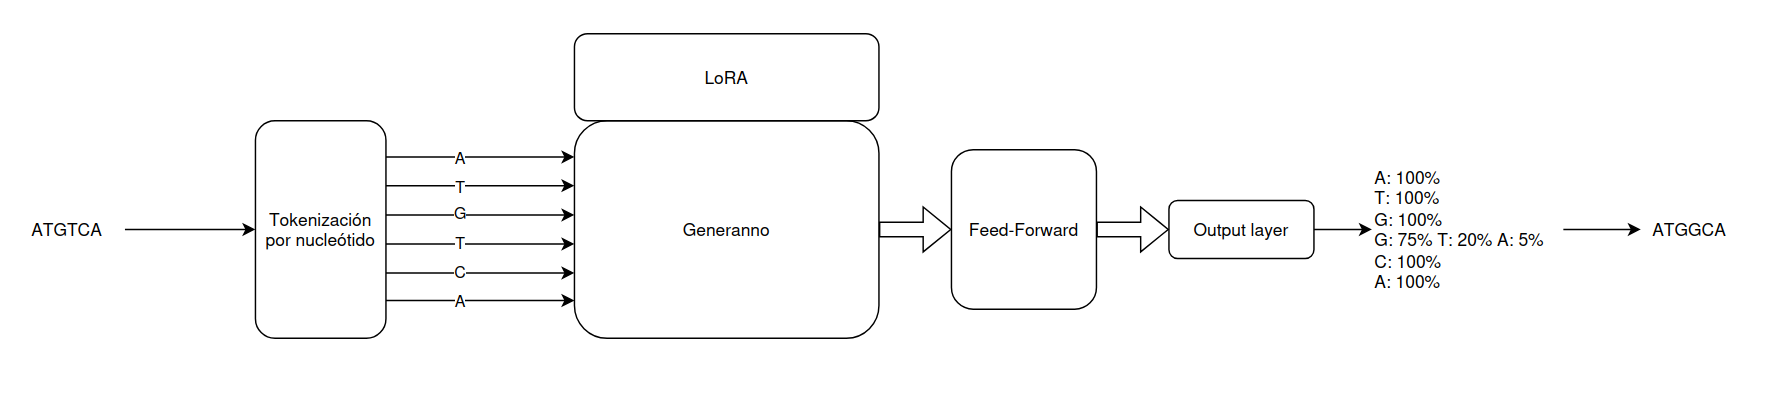
\includegraphics[width=\textwidth]{figuras/arquitectura.png}
  \caption{GENERanno ajustado con LoRA y una cabeza de clasificación}
  \Description{Diagrama de la arquitectura: la secuencia con errores entra a GENERanno con adaptadores LoRA y una cabeza de clasificación por posición que da la probabilidad de cada base.}
  \label{fig:arquitectura}
\end{figure*}

\subsection{Entrenamiento}\label{sec:entrenamiento}

Para entrenar el modelo propuesto se hizo un cambio a la entropía cruzada tradicional. Como el porcentaje de errores introducidos es muy bajo (como mucho, el 5 \%), de no darle más peso a la pérdida de esas posiciones, el modelo podría obtener una pérdida baja sin corregir nada, manteniendo todas las secuencias iguales. Por esto mismo se introdujo un hiperparámetro para controlar el peso de las posiciones con errores: las posiciones sin error tienen peso 1 y las posiciones con error, un peso w. Al calcular la pérdida promedio de un lote, la pérdida de cada posición se pondera con su peso y la suma se divide entre la suma de los pesos, lo que equivale a normalizar los pesos para que sumen 1, como se ve en la fórmula~\eqref{eq:perdida}. Los valores explorados para w fueron 1, 5, 20 y 100, donde w = 1 corresponde a la entropía cruzada estándar sin ponderar.
\begin{equation}\label{eq:perdida}
L = \frac{\sum_{i} v_{i} \cdot \mathrm{CE}_{i}}{\sum_{i} v_{i}}, \qquad v_{i} = \begin{cases} w & \text{si la posición } i \text{ tiene un error}\\ 1 & \text{de lo contrario} \end{cases}
\end{equation}

Respecto a la optimización de los modelos, se utilizó el optimizador AdamW con una tasa de aprendizaje máxima de 2 × 10⁻⁴ para todos los modelos e hiperparámetros probados. Al optimizador se le añadió decaimiento de pesos (weight decay), un parámetro que, entre más grande, más regulariza los pesos, reduciendo su tamaño antes de actualizarlos con el gradiente y sin modificar la función de pérdida. En cada paso, antes de la actualización de Adam, los pesos se multiplican por (1 − γλ), como se ve en la fórmula~\eqref{eq:wd}, donde γ es la tasa de aprendizaje y λ el decaimiento de pesos; después se aplica la actualización estándar de Adam. Esta reducción no pasa por el gradiente ni por los momentos de Adam, por lo que no se ve alterada por su tasa de aprendizaje adaptativa~\cite{pytorch_adamw}.
\begin{equation}\label{eq:wd}
\theta_{t} \leftarrow \theta_{t-1}(1-\gamma\lambda)
\end{equation}

Así se mejora la generalización del modelo~\cite{loshchilov2017decoupled}. El valor de este hiperparámetro fue 0.01 y se mantuvo fijo en todos los experimentos . Tanto la tasa de aprendizaje como el decaimiento de pesos se aplicaron solo a los parámetros entrenables, es decir, a las matrices de LoRA y a la cabeza de clasificación.

Al optimizador también se le aplicó un scheduler lineal con calentamiento, que, durante el primer 10 \% de los pasos de entrenamiento, incrementaba linealmente la tasa de aprendizaje desde 0 hasta su valor máximo (2 × 10⁻⁴) y, en el resto de los pasos, la reducía linealmente hasta 0. Cada paso corresponde a un lote, por lo que el total de pasos es el número de lotes por época multiplicado por el número de épocas. Esto se hace para evitar actualizaciones bruscas al inicio del entrenamiento, cuando la cabeza de clasificación todavía tiene pesos aleatorios y los gradientes son grandes y ruidosos~\cite{goyal2017accurate}. Luego, la tasa decrece para que el modelo, tras llegar rápido a una región adecuada del espacio de parámetros, pueda refinarlos~\cite{howard2018universal}.

El entrenamiento se realizó con lotes de 4 genes, un tamaño pequeño debido a limitaciones de recursos, un máximo de 5 épocas y parada temprana con paciencia de 2 épocas; es decir, si la ganancia en validación no mejoraba durante 2 épocas seguidas, el modelo detenía el entrenamiento y conservaba los pesos de la época con mejor ganancia en validación. Cada modelo se validó en la misma tasa y perfil de error con los que fue entrenado.

El criterio que se usó para elegir el mejor modelo e hiperparámetros fue la ganancia sobre el conjunto de validación, definida por Mitchell et al.~\cite{mitchell2020benchmarking} en la fórmula~\eqref{eq:ganancia-mitchell}. Esta vale 1 cuando se corrigen todos los errores sin introducir errores nuevos, es 0 cuando no se hacen cambios y puede ser negativa cuando se introducen más errores de los que se arreglan. La ganancia se calcula sobre todas las posiciones de todos los genes del conjunto, no gen por gen.
\begin{equation}\label{eq:ganancia-mitchell}
\mathrm{ganancia} = \frac{\text{errores corregidos} - \text{errores introducidos}}{\text{errores en la secuencia}}
\end{equation}

Por limitaciones de hardware, en lugar de explorar todas las combinaciones de rango de LoRA (4, 8 y 16), peso de error (1, 5, 20 y 100), perfil de error (uniforme y realista) y tasa de error (0.1 \%, 1 \% y 5 \%), que sumaban 72 configuraciones, se decidió hacer una exploración escalonada. Primero se exploraron los 4 pesos de error con un rango fijo de 8 y errores uniformes con una tasa de 1 \%. De ellos se eligió el peso con mayor ganancia en validación. Luego se probaron los rangos 4 y 16 con el mejor peso de error y la misma configuración de error, reutilizando el modelo de rango 8 ya entrenado, y se eligió el rango con mayor ganancia en validación. Finalmente, se entrenaron modelos en todas las tasas y perfiles de error usando el mejor rango y peso de error, por lo que en total solo hubo que entrenar 11 modelos. Para elegir el modelo final, cada uno de estos 6 modelos se evaluó sobre las 6 configuraciones de validación (3 tasas × 2 perfiles), y se eligió el de mayor ganancia media, usando el AUPRC medio como desempate. Así, el modelo elegido es el que mejor funciona cuando no se conoce de antemano la tasa ni el perfil de error real.

El entrenamiento se realizó en Google Colab con una GPU NVIDIA L4 (24 GB). Los pesos congelados del modelo base se cargaron en bfloat16, mientras que los adaptadores LoRA, la cabeza de clasificación y el cálculo de la pérdida se mantuvieron en float32. El tiempo promedio por época fue de 23.18 minutos, sin contar la evaluación en validación. Adicionalmente, para hacer un uso de memoria aún más eficiente, se activó el gradient checkpointing (puntos de control de gradientes): en vez de guardar todos los tensores intermedios de la pasada hacia adelante, se guardan solamente algunos y, cuando se necesitan los no guardados para calcular los gradientes, se recalcula un paso hacia adelante parcial. De esta forma se ahorra memoria, pero el entrenamiento tarda más~\cite{pytorch_checkpoint}.

La Tabla~\ref{tab:config} resume la configuración experimental del modelo propuesto, de la simulación de errores y de la línea base de N-gramas.

\begin{table}[t]
\caption{Configuración experimental}
\label{tab:config}
\footnotesize
\setlength{\tabcolsep}{4pt}
\begin{tabular}{@{}p{0.30\columnwidth}p{0.64\columnwidth}@{}}
\toprule
\textbf{Parámetro} & \textbf{Valor} \\
\midrule
\multicolumn{2}{@{}l}{\emph{Modelo}} \\
Modelo base & GENERanno-prokaryote-0.5b-base (28 capas, dimensión oculta de 1280, 16 cabezas de atención) \\
LoRA & Proyecciones de consulta, llave, valor y salida de la atención; $r \in \{4, 8, 16\}$ (elegido $r = 8$); $\alpha = 2r$ \\
Cabeza de clasificación & 1280 → 256 → 128 → 4, GELU, dropout de 0.1 \\
Parámetros entrenables & 2.23 millones con $r = 8$ (0.45 \% del modelo) \\
\midrule
\multicolumn{2}{@{}l}{\emph{Entrenamiento}} \\
Pérdida & Entropía cruzada ponderada, $w \in \{1, 5, 20, 100\}$ (elegido $w = 1$) \\
Optimizador & AdamW, tasa de aprendizaje máxima de 2 × 10⁻⁴, decaimiento de pesos de 0.01 \\
Scheduler & Calentamiento lineal en el primer 10 \% de los pasos y descenso lineal hasta 0 \\
Lote y épocas & 4 genes; máximo 5 épocas con parada temprana (paciencia de 2) \\
Selección & Ganancia en validación \\
Precisión y memoria & Pesos base en bfloat16; LoRA, cabeza y pérdida en float32; gradient checkpointing \\
Hardware & Google Colab, GPU NVIDIA L4 (24 GB) \\
\midrule
\multicolumn{2}{@{}l}{\emph{Errores simulados}} \\
Tasas y perfiles & 0.1 \%, 1 \% y 5 \%; uniforme y realista \\
Perfil realista & Lecturas de 150 nt, pendiente de 3, factor de 3 tras 3 o más bases iguales y 50 \% de repetición de la base anterior \\
Versiones con errores & 1 semilla en validación; 5 semillas en prueba y en arqueas \\
\midrule
\multicolumn{2}{@{}l}{\emph{Línea base de N-gramas}} \\
Rejilla & $N \in \{4, 7, 10, 13\}$, 4 patrones de pesos $\lambda$, $e \in \{0.1, 0.2, 0.3, 0.4\}$ \\
Elegido & $N = 4$, pesos lineales y $e = 0.1$ \\
\bottomrule
\end{tabular}
\end{table}

\subsection{Protocolo de evaluación}\label{sec:protocolo}

Para hacer la evaluación y comparación de los modelos se analizaron varios aspectos de las predicciones generadas por los modelos para los conjuntos de prueba de \emph{E. coli} y de arqueas. Las evaluaciones se realizaron posición por posición comparando la secuencia original, las versiones con errores que se usaron como entradas y las predicciones realizadas por el modelo. No hubo necesidad de hacer alineaciones entre estas secuencias, ya que solo hubo errores de sustitución de nucleótidos y las predicciones se entregan sin tokens de control y en formato de cadena de texto después de realizar la inferencia, por lo que tienen la misma longitud que la secuencia original.

\subsubsection{Métricas}\label{sec:metricas}

A continuación se presentan las métricas principales utilizadas para medir el rendimiento de los modelos sobre los conjuntos de validación y prueba. Vale la pena resaltar que no se calcula la exactitud, ya que un simple corrector que no hace ningún cambio tendría una exactitud de entre el 95 \% y el 99.9 \%, porque los errores o bases sustituidas son minoría en comparación con las bases sin cambios.

\begin{enumerate}

\item \emph{Detección (Precisión, Recall, F1):} para ver la capacidad de los modelos de encontrar errores, se definió el verdadero positivo de detección \(det_{TP}\ \)como las posiciones donde había un error y se hizo cualquier cambio en la predicción, sin importar si la base elegida era la correcta; el falso positivo \(det_{FP}\ \), como las posiciones donde no había errores y se hizo un cambio, y el falso negativo \(det_{FN}\ \), como las posiciones donde había un error y no se hizo ningún cambio. Las métricas usadas fueron la precisión~\eqref{eq:p-det}, el recall~\eqref{eq:r-det} y el F1~\eqref{eq:f1}, calculadas sobre todas las posiciones del conjunto.
\begin{align}
P &= \frac{\mathrm{det}_{TP}}{\mathrm{det}_{TP} + \mathrm{det}_{FP}} \label{eq:p-det}\\
R &= \frac{\mathrm{det}_{TP}}{\mathrm{det}_{TP} + \mathrm{det}_{FN}} \label{eq:r-det}\\
F1 &= \frac{2PR}{P + R} \label{eq:f1}
\end{align}

\item \emph{Correción (Precisión, Recall, F1):} para las correcciones, se definió el verdadero positivo \(corr_{TP}\ \) como las posiciones que tenían un error y se sustituyeron por el nucleótido correcto; el falso negativo \(corr_{FN}\ \), como las que tenían error y no se cambiaron o se cambiaron por otro nucleótido incorrecto, y los falsos positivos \(corr_{FP}\ \) se calcularon como el total de posiciones cambiadas por el modelo menos los verdaderos positivos, es decir, todos los cambios que no recuperan la base original, tanto en posiciones correctas como en posiciones con error. Para evaluar las capacidades de los modelos, se volvió a calcular la precisión~\eqref{eq:p-corr}, el recall~\eqref{eq:r-corr} y el F1~\eqref{eq:f1}, pero con las definiciones de corrección ya explicadas.
\begin{align}
P &= \frac{\mathrm{corr}_{TP}}{\mathrm{corr}_{TP} + \mathrm{corr}_{FP}} \label{eq:p-corr}\\
R &= \frac{\mathrm{corr}_{TP}}{\mathrm{corr}_{TP} + \mathrm{corr}_{FN}} \label{eq:r-corr}
\end{align}

\item \emph{Ganancia:} Aparte de la detección y corrección, la ganancia representa la métrica principal del proyecto y va muy de la mano con la corrección. Esta evalúa el modelo en términos de los errores que arregla (\(corr_{TP}\ \)), las posiciones correctas que modifica (\(det_{FP}\ \)) y el total de errores presentes en la secuencia de entrada, como se ve en la fórmula~\eqref{eq:ganancia}. Si se corrige todo y no se introducen errores, la ganancia será 1; si se corrigen tantos como se agregan, será 0; si no se corrige nada, será 0 también, y si es negativa, el modelo daña más la secuencia de lo que la arregla.
\begin{equation}\label{eq:ganancia}
\mathrm{Ganancia} = \frac{\mathrm{corr}_{TP} - \mathrm{det}_{FP}}{\#\ \text{de errores en la secuencia de entrada}}
\end{equation}

\item \emph{Sobrecorreción:} Algunos modelos tienden a cambiar muchas posiciones correctas por como están diseñados, por ejemplo, el modelo de n-gramas que, sin ningún tipo de control, busca el n-grama más probable y sustituye la base para todas las posiciones. Por esto, se evaluó la sobrecorrección como la proporción entre las posiciones dañadas por la predicción (\(\det_{FP}\)) y el total de posiciones en las que no se introdujeron errores, como se ve en la fórmula~\eqref{eq:sobrecorreccion}.
\begin{equation}\label{eq:sobrecorreccion}
\text{Sobrecorreción} = \frac{\mathrm{det}_{FP}}{\#\ \text{de posiciones sin error}}
\end{equation}

\item \emph{AUPRC:} AUPRC (área bajo la curva de precisión-recall): para el cálculo de este valor se toma 1 − P(base de entrada \textbar{} secuencia de entrada) para cada posición, representando una sospecha de error en esa posición. Luego, se ordenan todos estos valores de mayor a menor. Posteriormente, se calcula el average precision de esta lista, como se ve en la fórmula~\eqref{eq:ap}, donde \(P_{k}\) y \(R_{k}\)son la precisión y el recall al tomar las k primeras posiciones. Entonces, el AUPRC evalúa qué tan bien se ordenan y se ponen primero las posiciones con error en un ranking. Esta operación tiene sentido, ya que para el average precision se toman las posiciones donde incrementa en uno el recall, y como en esas posiciones el recall solo incrementa su numerador en una unidad, el incremento es solamente \(\frac{1}{|E|}\), donde \textbar E\textbar{} es el total de errores. Así, si se calcula el área bajo la curva de precisión-recall, en la cual se varía solamente el top-k que se toma, usando rectángulos, todos tendrían el mismo ancho \(\frac{1}{|E|}\), por lo que al final es solamente el promedio de las precisiones en los k donde se incrementa el recall. El AUPRC resume la precisión y el recall en un solo número sin importar el valor de k. Si el valor de AUPRC es 1, todos los errores reales quedaron arriba de todas las posiciones correctas en la lista, sin importar qué tan altas sean las probabilidades de sospecha de error.~\cite{sklearn_ap}
\begin{equation}\label{eq:ap}
AP = \sum_{k} (R_{k} - R_{k-1}) P_{k}
\end{equation}

\item \emph{\% de genes completamente correctos:} Otro valor fundamental para medir es qué tantos genes se corrigieron perfectamente, es decir, en cuántos la predicción quedó idéntica a la secuencia original, como se ve en la fórmula~\eqref{eq:genes}. Esto es importante saberlo porque la herramienta tendría su mayor utilidad entre más genes corrija perfectamente; de lo contrario, si no corrige muchos perfectamente, estaría cumpliendo solamente parcialmente con su objetivo.
\begin{equation}\label{eq:genes}
\%_{\mathrm{genes}} = \frac{\text{genes con predicción correcta}}{\text{total de genes}}
\end{equation}

\end{enumerate}

\subsubsection{Evaluación solo en las posiciones con error}\label{sec:oraculo}

Aparte de las métricas numéricas, también se hizo una modificación en la inferencia para evaluar otros aspectos del modelo. Se tomó la entrada y se evaluó solamente en las posiciones donde había errores, es decir, se asume que el modelo tiene una detección de errores perfecta y solo puede modificar la entrada en los sitios de error. Para esto, se tomó la base más probable distinta a la de la entrada y se midió el porcentaje de errores corregidos con la base original. Esto se hace con el objetivo de ver qué tanto se está fallando por la detección y qué tanto se está fallando por la corrección individualmente. La idea se tomó de Zhang et al.~\cite{zhang2020spelling}, en el cual se hacía lo mismo para ver el límite superior que podían alcanzar en el caso de tener una detección perfecta. Esta evaluación se puede comparar directamente con el corrector por frecuencia que se propuso como línea base, ya que este usa este mismo escenario, pero elige la base al azar ponderando por la frecuencia de cada nucleótido en los datos de entrenamiento. Otro punto de comparación es el azar uniforme, que acertaría en el 33 \% de sus predicciones al asignar la misma probabilidad a los tres nucleótidos restantes.

\subsubsection{Evaluación a nivel de codón y por categorías}\label{sec:categorias}

Otras formas de evaluación realizadas fueron a nivel de codón y por características especiales. Se calcularon: ganancia, precisión/recall/F1 de detección, recall/F1 de corrección, sobrecorrección (sobre las posiciones correctas de esa posición) y exactitud con oráculo, para cada una de las 3 posiciones de los codones para ver si hay alguna tendencia en las correcciones de los modelos. Además, se calcularon el recall de detección, el recall de corrección y la exactitud con oráculo agrupando los errores según su efecto en la proteína: sinónimos, si el codón con error codifica el mismo aminoácido; no sinónimos, si codifica otro aminoácido, y sin sentido, si crea un codón de parada prematuro. Esto permite ver si el modelo detecta mejor los errores que más alteran la proteína. Con las mismas métricas, los errores también se agruparon por tipo de sustitución, separando las transiciones (A↔G y C↔T) de las transversiones (las otras ocho sustituciones). También se hizo un análisis en el cual se calcularon las frecuencias de las sustituciones hechas por el modelo, es decir, con qué frecuencia se cambia un nucleótido por otro específico. Por último, se revisó que se acertaran las correcciones en los nucleótidos de los codones de inicio y parada, ya que esta corrección debería ser más sencilla porque en esas posiciones hay muy pocos codones posibles, y así podemos revisar que el modelo haya capturado este aspecto fundamental del lenguaje del ADN. Finalmente, se calculó la ganancia del modelo ajustado agrupando los genes por su contenido de GC, y se evaluaron los 6 modelos finales en las 6 configuraciones de prueba para comparar la tasa de entrenamiento con la de evaluación.

\subsubsection{Conjunto de prueba}\label{sec:conjunto-prueba}

Vale la pena resaltar que para evaluar el conjunto de prueba y el conjunto de genes de arqueas, como se explicó previamente, se generaron 5 versiones con errores con diferentes semillas para todas las combinaciones de tasa y perfil de errores consideradas. Esto se hizo con el fin de calcular las métricas ya exploradas en cada versión y reportar su media y desviación estándar.

\subsubsection{Intervalos de confianza del 95\%}\label{sec:intervalos}

Para evaluar la estabilidad de los resultados, se realizó el cálculo de intervalos de confianza por bootstrap. Se crearon 1000 conjuntos del mismo tamaño que el conjunto de prueba combinado a traves de sus 5 versiones dependientes de la semilla, tomando genes completos aleatoriamente y con reemplazo de este. En cada uno se calcularon las métricas y luego los percentiles 2.5 y 97.5 de los valores obtenidos, que son los límites del intervalo de confianza del 95 \%, lo que permite medir qué tanto dependen los resultados de los genes que se toman. Se remuestrearon genes completos y no posiciones individuales, porque las posiciones de un mismo gen no son independientes. Para comparar dos modelos se usó el mismo remuestreo en ambos y se calculó el intervalo de la diferencia de sus métricas.

\subsubsection{Criterios de éxito}\label{sec:criterios}

Antes de ver los resultados del conjunto de prueba se definieron los siguientes criterios de éxito:

\begin{enumerate}
\renewcommand{\labelenumi}{\alph{enumi}.}

\item Conseguir una ganancia mayor a 0 en todas las tasas y perfiles, con el límite inferior de su intervalo de confianza mayor que 0, lo que significa que se hacen sustituciones que en efecto corrigen el gen y que estas correcciones son más que los errores introducidos.

\item Superar la línea base de n-gramas en F1 de detección, F1 de corrección, con un intervalo de confianza de la diferencia que no incluya el 0.

\item Obtener una ganancia mayor a 0 en los conjuntos de prueba de arqueas, con el mismo criterio.

\end{enumerate}

\section{Resultados}\label{sec:resultados}

En esta sección se presentan los resultados obtenidos siguiendo el protocolo de evaluación descrito en la sección~\ref{sec:protocolo}. Primero se reporta la selección de hiperparámetros y del modelo final, que se hizo únicamente con el conjunto de validación; luego, los resultados de todos los modelos sobre el conjunto de prueba de \emph{E. coli} y sobre los genes de \emph{H. volcanii}, y, finalmente, los análisis complementarios a nivel de gen, de codón, por categorías y por tasa de entrenamiento. Salvo que se indique lo contrario, los valores corresponden a la media ± la desviación estándar sobre las 5 versiones con errores de cada configuración. Antes de evaluar se verificó que la partición de genes fuera exactamente la misma con la que se entrenaron y seleccionaron los modelos (3,407 genes de entrenamiento, 415 de validación y 433 de prueba). Como la diferencia entre los perfiles uniforme y realista fue muy pequeña para el modelo propuesto (como mucho 0.012 de ganancia en \emph{E. coli} y 0.003 en arqueas), en las tablas se reporta el perfil realista, y el uniforme se menciona solo cuando cambia alguna conclusión.

\subsection{Selección de hiperparámetros y del modelo final}\label{sec:res-seleccion}

Para el modelo de N-gramas, de las 64 combinaciones exploradas la de mayor ganancia media en validación fue N = 4 (un codón de contexto a cada lado) con pesos lineales y e = 0.1, con una ganancia media de apenas 0.0007. Las combinaciones con contextos más largos y con pesos que favorecen los órdenes altos obtuvieron ganancias muy negativas (hasta −149.9 con N = 13, pesos geométricos y e = 0.4), ya que cambian muchas más posiciones correctas de las que corrigen. Vale la pena resaltar que e = 0.1 es el menor valor explorado, es decir, el más conservador.

Para el modelo propuesto, en la primera etapa de la exploración (rango 8 y errores uniformes del 1 \%) la ganancia en validación disminuyó a medida que aumentaba el peso de las posiciones con error: 0.880 con w = 1, 0.838 con w = 5, 0.684 con w = 20 y 0.316 con w = 100, por lo que se eligió w = 1, es decir, la entropía cruzada sin ponderar. En la segunda etapa, los rangos 4, 8 y 16 obtuvieron ganancias de 0.879, 0.880 y 0.874, respectivamente; como la diferencia entre ellos es menor a 0.006, se mantuvo el rango 8. Finalmente, al evaluar los 6 modelos finales sobre las 6 configuraciones de validación, el de mayor ganancia media fue el entrenado con errores realistas del 1 \% (ganancia media de 0.726 y AUPRC media de 0.965), seguido por los de 1 \% uniforme (0.695), 0.1 \% realista (0.673), 0.1 \% uniforme (0.637), 5 \% realista (0.467) y 5 \% uniforme (0.448). Este es el modelo que se reporta como «ajustado» en el resto de la sección. Cada uno de los 11 modelos tardó cerca de 1.9 horas en entrenarse (21.2 horas de GPU en total), y en 4 de ellos la mejor época fue la última.

La Fig.~\ref{fig:curvas} muestra la evolución por época de la pérdida y de las métricas de validación para cada peso. Con w = 1 la ganancia fue la más alta en todas las épocas y su mejor época fue la quinta (0.8796); con w = 5, w = 20 y w = 100 las mejores épocas fueron la tercera (0.8376), la cuarta (0.6839) y la cuarta (0.3163). En cambio, el AUPRC de los cuatro pesos terminó entre 0.981 y 0.984.

\begin{figure*}[p]
  \centering
  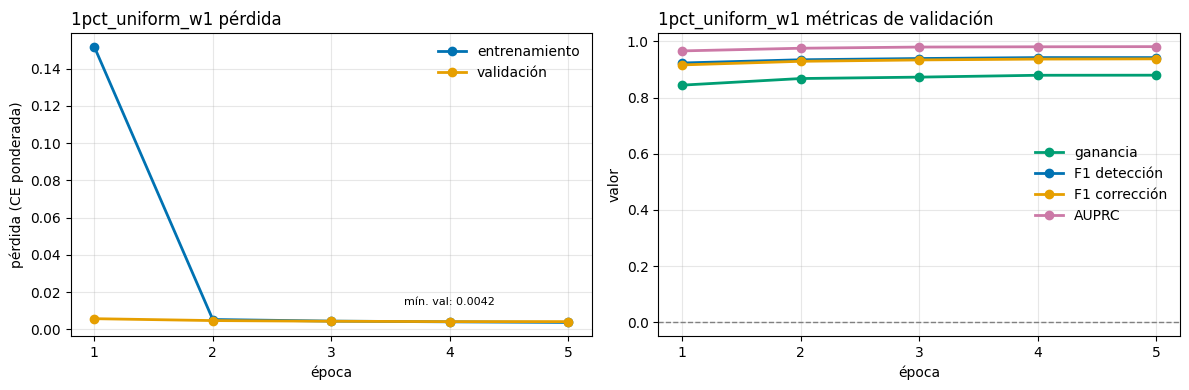
\includegraphics[width=0.76\textwidth]{figuras/fig_curvas_w1.png}\\(a) $w = 1$\\[4pt]
  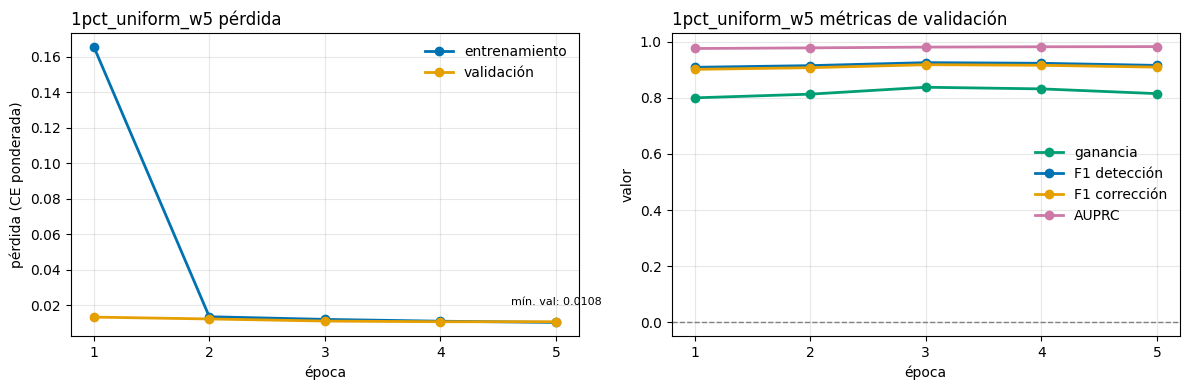
\includegraphics[width=0.76\textwidth]{figuras/fig_curvas_w5.png}\\(b) $w = 5$\\[4pt]
  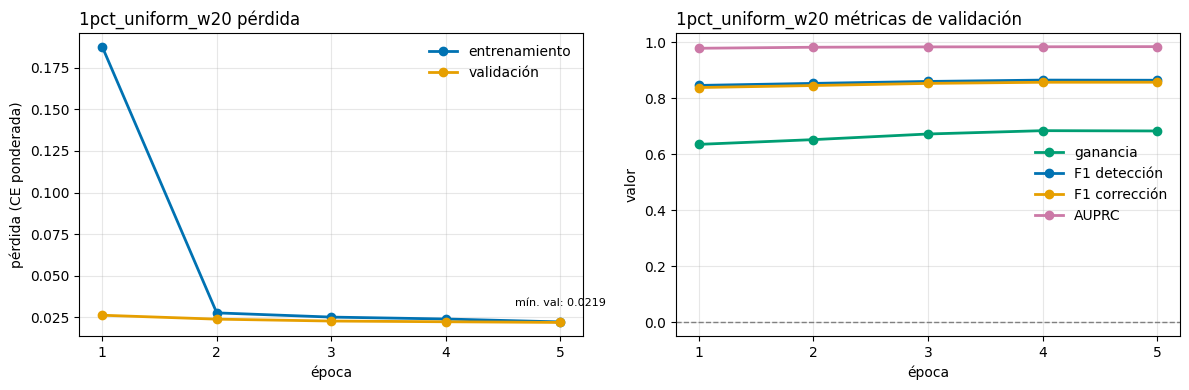
\includegraphics[width=0.76\textwidth]{figuras/fig_curvas_w20.png}\\(c) $w = 20$\\[4pt]
  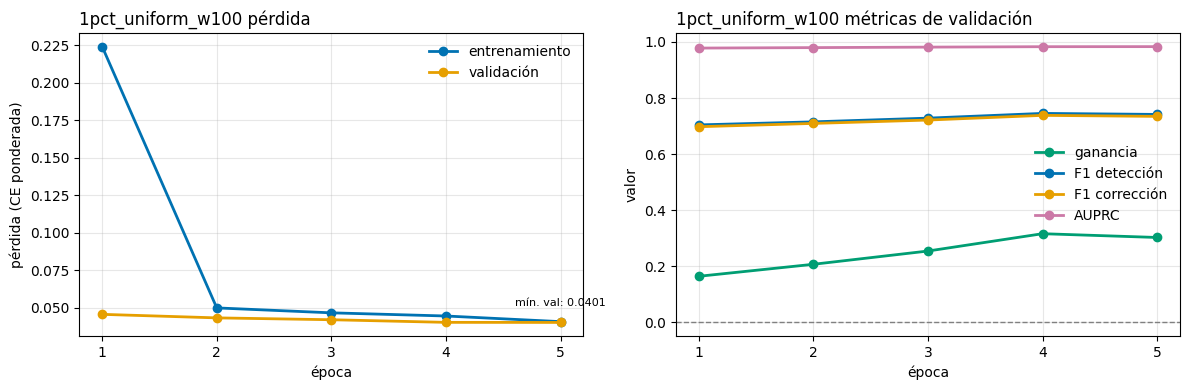
\includegraphics[width=0.76\textwidth]{figuras/fig_curvas_w100.png}\\(d) $w = 100$
  \caption{Curvas de entrenamiento por época para los cuatro pesos del error explorados (rango 8 y errores uniformes del 1 \%). En cada panel, la izquierda muestra la pérdida de entrenamiento y de validación, y la derecha la ganancia, el F1 de detección, el F1 de corrección y el AUPRC en validación.}
  \Description{Cuatro pares de gráficas de líneas por época. La pérdida de entrenamiento cae fuertemente después de la primera época y la de validación se mantiene baja; la ganancia en validación es mayor con w igual a 1 y mucho menor con w igual a 100, mientras que el AUPRC queda cerca de 0.98 en los cuatro casos.}
  \label{fig:curvas}
\end{figure*}

\subsection{Resultados en el conjunto de prueba de \emph{E. coli}}\label{sec:res-prueba}

La Tabla~\ref{tab:prueba} resume las métricas principales sobre el conjunto de prueba de \emph{E. coli}, y la Fig.~\ref{fig:ganancia}a muestra la ganancia en función de la tasa de error. El modelo ajustado obtuvo la mayor ganancia en todas las tasas: 0.413 ± 0.030 con errores del 0.1 \%, 0.878 ± 0.006 con el 1 \% y 0.818 ± 0.003 con el 5 \%. Con el 1 \%, que es la tasa con la que se entrenó, corrigió el 93.1 \% de los errores, con una precisión de detección de 0.946 y un recall de detección de 0.937. Con el 5 \% la precisión subió a 0.984, pero el recall bajó a 0.842, es decir, el modelo dejó más errores sin detectar. Con el 0.1 \% ocurrió lo contrario: el recall de detección fue de 0.951, pero la precisión bajó a 0.640, lo que redujo la ganancia a menos de la mitad.

\begin{table*}[t]
\caption{Resultados en el conjunto de prueba de E. coli (perfil realista)}
\label{tab:prueba}
\small
\begin{tabular}{llrrrrr}
\toprule
\textbf{Modelo} & \textbf{Tasa} & \textbf{Ganancia} & \textbf{F1 det.} & \textbf{F1 corr.} & \textbf{Sobrecorr. (×10\textsuperscript{−3})} & \textbf{AUPRC} \\
\midrule
Sin cambios & 0.1 \% & 0.000 ± 0.000 & 0.000 & 0.000 & 0.00 & 0.001 \\
 & 1 \% & 0.000 ± 0.000 & 0.000 & 0.000 & 0.00 & 0.010 \\
 & 5 \% & 0.000 ± 0.000 & 0.000 & 0.000 & 0.00 & 0.050 \\
\midrule
Frecuencia* & 0.1 \% & 0.335 ± 0.029 & --- & 0.335 & --- & --- \\
 & 1 \% & 0.331 ± 0.005 & --- & 0.331 & --- & --- \\
 & 5 \% & 0.333 ± 0.004 & --- & 0.333 & --- & --- \\
\midrule
N-gramas & 0.1 \% & 0.000 ± 0.000 & 0.000 & 0.000 & 0.00 & 0.002 \\
 & 1 \% & 0.001 ± 0.001 & 0.002 & 0.001 & 0.00 & 0.021 \\
 & 5 \% & 0.001 ± 0.000 & 0.001 & 0.001 & 0.00 & 0.090 \\
\midrule
Zero-shot & 0.1 \% & −4.088 ± 0.167 & 0.227 & 0.223 & 4.68 & 0.666 \\
 & 1 \% & 0.232 ± 0.014 & 0.654 & 0.644 & 4.77 & 0.746 \\
 & 5 \% & 0.440 ± 0.008 & 0.676 & 0.660 & 6.16 & 0.707 \\
\midrule
Ajustado & 0.1 \% & 0.413 ± 0.030 & 0.765 & 0.762 & 0.52 & 0.919 \\
 & 1 \% & 0.878 ± 0.006 & 0.942 & 0.936 & 0.54 & 0.975 \\
 & 5 \% & 0.818 ± 0.003 & 0.907 & 0.897 & 0.73 & 0.977 \\
\bottomrule
\end{tabular}

\vspace{2pt}\begin{minipage}{\textwidth}\footnotesize Media ± desviación estándar de la ganancia sobre las 5 semillas; para las demás métricas se muestra la media (desviaciones ≤ 0.03). *El corrector por frecuencia conoce la posición de los errores, por lo que sus métricas de detección, su sobrecorrección y su AUPRC no aplican. El AUPRC del azar es igual a la tasa de error, que es el valor que obtiene el corrector sin cambios.\end{minipage}
\end{table*}

Esta caída no se debe a que el modelo cambie más posiciones correctas cuando hay pocos errores. La sobrecorrección del modelo ajustado se mantuvo casi constante, entre 0.52 × 10\textsuperscript{−3} y 0.73 × 10\textsuperscript{−3}, lo que equivale a un cambio indebido por cada 1,360 a 1,930 posiciones correctas. En números absolutos, el modelo introdujo en promedio 215, 221 y 290 errores por versión del conjunto de prueba con las tasas de 0.1 \%, 1 \% y 5 \%, mientras que el número de errores simulados fue de 403, 4,138 y 20,862, respectivamente. Así, con el 0.1 \% los errores introducidos equivalen a más de la mitad de los errores que hay que corregir y pesan mucho en la ganancia, mientras que con el 1 \% y el 5 \% son una fracción pequeña.

GENERanno sin ajuste (zero-shot) detectó una buena parte de los errores (recall de detección de 0.746 con el 0.1 \% y de 0.717 con el 1 \%), pero su sobrecorrección fue cerca de 9 veces la del modelo ajustado (entre 4.7 × 10\textsuperscript{−3} y 6.2 × 10\textsuperscript{−3}) y, como también se mantuvo casi constante, su ganancia cambió de signo según la tasa: −4.088 con el 0.1 \%, 0.232 con el 1 \% y 0.440 con el 5 \%. Con el 0.1 \%, por ejemplo, introdujo en promedio 1,941 errores por versión del conjunto para corregir 295 de los 403 errores simulados.

El modelo de N-gramas casi no hizo cambios: su recall de detección fue como mucho de 0.001 y su ganancia no superó 0.001 en ninguna configuración, aunque cuando hizo un cambio casi siempre fue en una posición con error (precisión de detección entre 0.93 y 1.00). Aun así, su AUPRC (0.002, 0.021 y 0.090) fue cerca del doble de la del azar (0.001, 0.010 y 0.050), lo que indica que sus probabilidades sí ordenan parcialmente los errores, pero casi nunca superan el costo de cambiar una base que impone e. El corrector por frecuencia, que conoce la posición de los errores, corrigió entre el 33.1 \% y el 34.3 \% de ellos, prácticamente lo mismo que elegir al azar entre las tres bases restantes. Por último, el corrector sin cambios obtuvo una ganancia de 0 y un AUPRC igual a la tasa de error, como se esperaba por construcción, lo que sirvió también como verificación del cálculo de las métricas. En AUPRC, el modelo ajustado obtuvo 0.919, 0.975 y 0.977, muy por encima del zero-shot (0.666, 0.746 y 0.707).

\begin{figure*}[t]
  \centering
  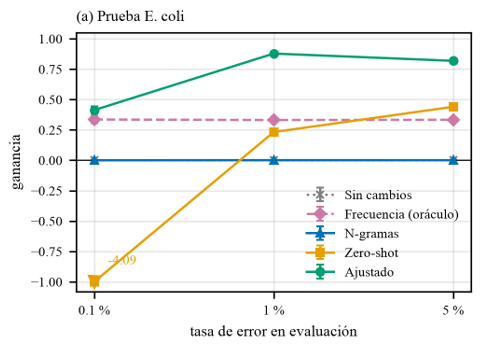
\includegraphics[width=0.49\textwidth]{figuras/fig2a_ganancia_prueba.png}\hfill
  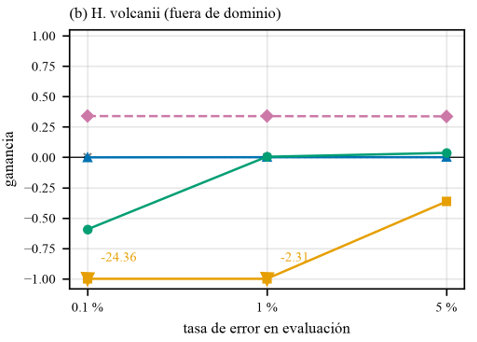
\includegraphics[width=0.49\textwidth]{figuras/fig2b_ganancia_hvolcanii.png}
  \caption{Ganancia en función de la tasa de error en evaluación, con el perfil realista, en (a) el conjunto de prueba de \emph{E. coli} y (b) los genes de \emph{H. volcanii}. Las barras muestran la desviación estándar sobre las 5 semillas. Los valores del zero-shot menores a −1 se indican con un triángulo y su valor. La línea del corrector sin cambios queda bajo la del N-gramas, ya que ambas están en 0.}
  \Description{Dos gráficas de líneas de la ganancia de cada modelo frente a la tasa de error de evaluación (0.1 \%, 1 \% y 5 \%), una para la prueba de E. coli y otra para H. volcanii.}
  \label{fig:ganancia}
\end{figure*}

\subsection{Resultados fuera de dominio (\emph{H. volcanii})}\label{sec:res-arqueas}

En las arqueas, el desempeño de todos los modelos cayó de forma marcada (Tabla~\ref{tab:arqueas} y Fig.~\ref{fig:ganancia}b). Con tasas de error simuladas del 0.1 \%, 1 \% y 5 \%, el modelo ajustado obtuvo ganancias de −0.593 ± 0.007, 0.004 ± 0.002 y 0.036 ± 0.0005, respectivamente. La caída se debe sobre todo a la detección: el modelo encontró menos del 10 \% de los errores (recall de detección de 0.096, 0.089 y 0.063), mientras que su sobrecorrección (entre 0.68 × 10−3 y 0.97 × 10−3) fue solo algo mayor que en E. coli. Con el 0.1 \%, por ejemplo, cada versión del conjunto de arqueas tenía en promedio 3,365 errores: el modelo corrigió 276, pero cambió 2,273 posiciones que estaban correctas, por lo que su ganancia fue negativa, (276 − 2,273) / 3,365 = −0.593. Es decir, con esa tasa las secuencias quedaron con más errores de los que tenían antes de corregirlas. El zero-shot obtuvo ganancias negativas en todas las tasas (−24.36, −2.31 y −0.37), con una sobrecorrección de 2.5 × 10−2, cinco veces la que tuvo en E. coli. El N-gramas volvió a quedar cerca de 0 (entre −0.001 y 0.001) y el corrector por frecuencia corrigió entre el 32.9 \% y el 33.9 \% de los errores. En AUPRC, el modelo ajustado (0.051, 0.157 y 0.277) siguió por encima del zero-shot (0.014, 0.066 y 0.145) y del azar, pero muy lejos de los valores que obtuvo en E. coli.

\begin{table*}[t]
\caption{Resultados en los genes de H. volcanii, fuera de dominio (perfil realista)}
\label{tab:arqueas}
\small
\begin{tabular}{llrrrrr}
\toprule
\textbf{Modelo} & \textbf{Tasa} & \textbf{Ganancia} & \textbf{F1 det.} & \textbf{F1 corr.} & \textbf{Sobrecorr. (×10\textsuperscript{−3})} & \textbf{AUPRC} \\
\midrule
Sin cambios & 0.1 \% & 0.000 ± 0.000 & 0.000 & 0.000 & 0.00 & 0.001 \\
 & 1 \% & 0.000 ± 0.000 & 0.000 & 0.000 & 0.00 & 0.010 \\
 & 5 \% & 0.000 ± 0.000 & 0.000 & 0.000 & 0.00 & 0.050 \\
\midrule
Frecuencia* & 0.1 \% & 0.339 ± 0.012 & --- & 0.339 & --- & --- \\
 & 1 \% & 0.338 ± 0.002 & --- & 0.338 & --- & --- \\
 & 5 \% & 0.337 ± 0.001 & --- & 0.337 & --- & --- \\
\midrule
N-gramas & 0.1 \% & −0.001 ± 0.001 & 0.002 & 0.001 & 0.00 & 0.002 \\
 & 1 \% & 0.001 ± 0.000 & 0.002 & 0.001 & 0.00 & 0.017 \\
 & 5 \% & 0.001 ± 0.000 & 0.002 & 0.001 & 0.00 & 0.073 \\
\midrule
Zero-shot & 0.1 \% & −24.360 ± 0.426 & 0.014 & 0.010 & 24.57 & 0.014 \\
 & 1 \% & −2.309 ± 0.014 & 0.096 & 0.074 & 24.65 & 0.066 \\
 & 5 \% & −0.365 ± 0.003 & 0.179 & 0.133 & 24.87 & 0.145 \\
\midrule
Ajustado & 0.1 \% & −0.593 ± 0.007 & 0.108 & 0.092 & 0.68 & 0.051 \\
 & 1 \% & 0.004 ± 0.002 & 0.153 & 0.133 & 0.73 & 0.157 \\
 & 5 \% & 0.036 ± 0.0005 & 0.117 & 0.100 & 0.97 & 0.277 \\
\bottomrule
\end{tabular}

\vspace{2pt}\begin{minipage}{\textwidth}\footnotesize Tasa: porcentaje de posiciones con error simulado en la secuencia de entrada. Mismo formato que la Tabla~\ref{tab:prueba}. *Frecuencia conoce la posición de los errores.\end{minipage}
\end{table*}

\subsection{Detección perfecta (oráculo)}\label{sec:res-oraculo}

Al evaluar solo en las posiciones con error, eligiendo la base más probable distinta de la de entrada (Tabla~\ref{tab:oraculo}), el modelo ajustado acertó en el 98.5 \% de los errores con el 1 \%, frente al 93.1 \% que corrige cuando tiene que detectarlos por sí mismo; con el 0.1 \% y el 5 \% acertó en el 98.6 \% y el 97.1 \%. Es decir, en \emph{E. coli} casi todo lo que el modelo deja de corregir se pierde en la detección y no en la elección de la base. El zero-shot acertó en el 90.5 \% de los errores, muy por encima del 70.6 \% que corrige sin oráculo; el N-gramas, en el 47.2 \%, y el corrector por frecuencia, en el 33.1 \%, cerca del 33.3 \% que se obtendría al azar. En las arqueas la brecha fue mucho mayor: con oráculo, el modelo ajustado acertó en el 67.4 \% de los errores, pero sin oráculo solo corrigió el 7.7 \%; el zero-shot acertó en el 62.4 \%, el N-gramas en el 39.0 \% y el corrector por frecuencia en el 33.8 \%. Los resultados a nivel de codón fueron prácticamente iguales (por ejemplo, 98.4 \% para el modelo ajustado en \emph{E. coli} con el 1 \%), ya que casi ningún codón tiene más de un error.

\begin{table}[t]
\caption{Corrección sin oráculo y con oráculo, con el 1 \% de errores (perfil realista)}
\label{tab:oraculo}
\footnotesize
\setlength{\tabcolsep}{3pt}
\begin{tabular}{lrrrr}
\toprule
 & \multicolumn{2}{c}{\textbf{Prueba E. coli}} & \multicolumn{2}{c}{\textbf{H. volcanii}} \\
\cmidrule(lr){2-3}\cmidrule(lr){4-5}
\textbf{Modelo} & \textbf{\shortstack[r]{Recall\\corr. (\%)}} & \textbf{\shortstack[r]{Con\\oráculo (\%)}} & \textbf{\shortstack[r]{Recall\\corr. (\%)}} & \textbf{\shortstack[r]{Con\\oráculo (\%)}} \\
\midrule
Frecuencia* & 33.1 & 33.1 & 33.8 & 33.8 \\
N-gramas & 0.1 & 47.2 & 0.1 & 39.0 \\
Zero-shot & 70.6 & 90.5 & 13.4 & 62.4 \\
Ajustado & 93.1 & 98.5 & 7.7 & 67.4 \\
\bottomrule
\end{tabular}

\vspace{2pt}\parbox{\columnwidth}{\footnotesize Recall de corrección: errores corregidos por el modelo con su propia detección. Con oráculo: errores corregidos si el modelo elige la base más probable distinta de la de entrada solo en las posiciones con error. *En Frecuencia ambos valores coinciden, ya que siempre conoce la posición de los errores.}
\end{table}

\subsection{Exactitud a nivel de gen}\label{sec:res-gen}

Con el 0.1 \% de errores, 198 de los 433 genes de prueba (45.7 \%) no recibieron ningún error, por lo que el corrector sin cambios ya los deja perfectos (Tabla~\ref{tab:genes}). De los 235 genes que sí tenían errores, el modelo ajustado dejó idénticos al original el 61.4 \% (cerca de 144 genes), pero de los 198 genes sin errores dañó el 35.2 \% (cerca de 70). En total quedaron perfectos 198 − 70 + 144 ≈ 272 genes, el 62.9 \% del conjunto, frente al 45.7 \% del corrector sin cambios. Con el 1 \%, solo el 2.6 \% de los genes quedó sin errores y el modelo ajustado dejó perfectos el 39.7 \%; con el 5 \%, apenas el 1.2 \%. El zero-shot dañó el 69.0 \% de los genes sin errores con el 0.1 \%, por lo que dejó perfectos solo el 15.1 \%, menos de la tercera parte de lo que deja el corrector sin cambios. En las arqueas, con el 0.1 \%, el modelo ajustado dejó perfectos el 40.8 \% de los genes, por debajo del 47.4 \% del corrector sin cambios: reparó solo el 2.0 \% de los genes con errores y dañó el 16.2 \% de los que no tenían.

\begin{table*}[t]
\caption{Porcentaje de genes de prueba de E. coli perfectos, reparados y dañados (perfil realista)}
\label{tab:genes}
\small
\begin{tabular}{lrrrrrr}
\toprule
 & \multicolumn{3}{c}{\textbf{0.1 \% de errores}} & \multicolumn{3}{c}{\textbf{1 \% de errores}} \\
\cmidrule(lr){2-4}\cmidrule(lr){5-7}
\textbf{Modelo} & \textbf{Perfectos} & \textbf{Reparados} & \textbf{Dañados} & \textbf{Perfectos} & \textbf{Reparados} & \textbf{Dañados} \\
\midrule
Sin cambios & 45.7 & 0.0 & 0.0 & 2.6 & 0.0 & 0.0 \\
Frecuencia* & 57.0 & 20.8 & 0.0 & 5.1 & 2.5 & 0.0 \\
Zero-shot & 15.1 & 1.7 & 69.0 & 2.9 & 0.4 & 5.2 \\
Ajustado & 62.9 & 61.4 & 35.2 & 39.7 & 38.6 & 20.2 \\
\bottomrule
\end{tabular}

\vspace{2pt}\begin{minipage}{\textwidth}\footnotesize Cada columna se calcula sobre un grupo distinto de genes. Perfectos: porcentaje de todos los genes de prueba (433) que quedan idénticos al original después de corregir. Reparados: porcentaje de los genes que tenían al menos un error que quedan idénticos al original. Dañados: porcentaje de los genes que no tenían errores en los que el modelo introdujo al menos uno. La fila Sin cambios indica cuántos genes no recibieron errores (45.7 \% con el 0.1 \% y 2.6 \% con el 1 \%). Con el 1 \% solo cerca de 11 genes no reciben errores, por lo que el porcentaje de dañados es poco estable.\end{minipage}
\end{table*}

\subsection{Nivel de codón y posición en el codón}\label{sec:res-codon}

A nivel de codón, las métricas fueron muy similares a las de nucleótido; por ejemplo, la ganancia del modelo ajustado fue de 0.416, 0.879 y 0.820 con las tres tasas. Al separar por la posición del nucleótido en el codón (Fig.~\ref{fig:posicion}), la tercera posición fue la más difícil para los dos modelos basados en GENERanno. Con el 1 \% y juntando ambos perfiles, el recall de detección del modelo ajustado fue de 0.953, 0.966 y 0.889 en la primera, segunda y tercera posición, y su sobrecorrección en la tercera (0.88 × 10\textsuperscript{−3}) fue más del doble que en las otras dos (0.38 × 10\textsuperscript{−3} y 0.34 × 10\textsuperscript{−3}). Como consecuencia, su ganancia en la tercera posición fue de 0.792, frente a 0.912 y 0.930, y con el 0.1 \% llegó a ser negativa (−0.080 ± 0.086, frente a 0.633 y 0.677). El zero-shot mostró el mismo patrón de forma más marcada (ganancias de 0.360, 0.482 y −0.138 con el 1 \%). Con oráculo, en cambio, la diferencia entre posiciones fue pequeña (98.9 \%, 99.2 \% y 97.5 \%), por lo que la dificultad de la tercera posición está en la detección. En las arqueas, el recall de detección del modelo ajustado con el 1 \% fue de 0.094, 0.133 y 0.043, es decir, también el más bajo en la tercera posición.

\begin{figure*}[t]
  \centering
  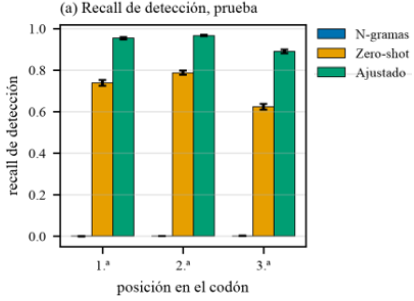
\includegraphics[width=0.32\textwidth]{figuras/fig3a_recall_posicion_prueba.png}\hfill
  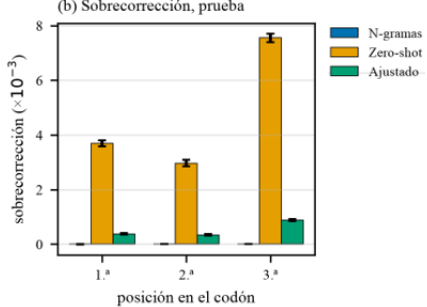
\includegraphics[width=0.32\textwidth]{figuras/fig3b_sobrecorreccion_posicion_prueba.png}\hfill
  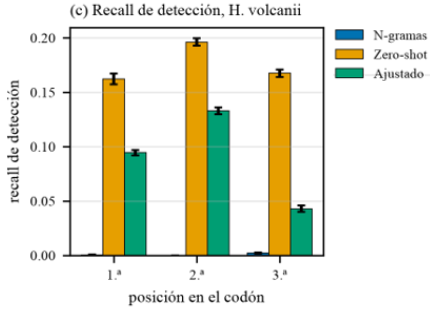
\includegraphics[width=0.32\textwidth]{figuras/fig3c_recall_posicion_hvolcanii.png}
  \caption{Métricas por posición del nucleótido en el codón con el 1 \% de errores (ambos perfiles y las 5 semillas; las barras de error son la desviación estándar sobre esas 10 configuraciones): (a) recall de detección y (b) sobrecorrección en el conjunto de prueba de \emph{E. coli}, y (c) recall de detección en \emph{H. volcanii}. Las barras del N-gramas son cercanas a 0.}
  \Description{Tres gráficas de barras por posición en el codón (1.ª, 2.ª y 3.ª) para N-gramas, zero-shot y el modelo ajustado.}
  \label{fig:posicion}
\end{figure*}

\subsection{Desglose por categorías}\label{sec:res-categorias}

Para ver qué errores le cuestan más a cada modelo, los errores del conjunto de prueba con el 1 \% se separaron en grupos y, en cada grupo, se calculó qué porcentaje de ellos detectó y corrigió cada modelo (Tabla~\ref{tab:categorias}). Se usaron tres agrupaciones. La primera es el efecto del error en la proteína: un error es sinónimo si el codón con error codifica el mismo aminoácido que el original (por ejemplo, CTG → CTA, ambos leucina), no sinónimo si codifica otro aminoácido (por ejemplo, GAA → GAT, de ácido glutámico a ácido aspártico) y sin sentido si convierte el codón en uno de parada (por ejemplo, TGG → TGA, de triptófano a parada), lo que cortaría la proteína. La segunda es el tipo de sustitución: las bases se dividen en purinas (A y G) y pirimidinas (C y T); una transición cambia una base por otra del mismo tipo (A↔G o C↔T) y una transversión, por una del otro tipo (por ejemplo, A↔C o G↔T). Como cada base tiene una transición posible y dos transversiones, hay 4 transiciones y 8 transversiones. La tercera es la ubicación del error: el codón de inicio, el de parada o el interior del gen.

El modelo ajustado detectó el 98.5 \% de los errores sin sentido, el 96.0 \% de los no sinónimos y solo el 85.6 \% de los sinónimos. Con oráculo estas diferencias casi desaparecen (99.1 \%, 98.8 \% y 97.7 \%); es decir, cuando el modelo sabe dónde está el error, elige bien la base en los tres grupos, y la dificultad de los errores sinónimos está en notar que hay un error. El zero-shot siguió el mismo orden, con valores más bajos (90.2 \%, 74.9 \% y 59.0 \%). Las transiciones se detectaron menos que las transversiones (90.3 \% frente a 95.3 \%); cada una de las cuatro transiciones tuvo un recall de detección entre 89.3 \% y 90.9 \%, y cada una de las ocho transversiones, entre 94.8 \% y 96.1 \%. Por ubicación, los errores en el codón de inicio y en el de parada se detectaron menos que los del interior del gen (77.6 \% y 76.3 \% frente a 93.7 \%), aunque estos dos grupos tienen pocos errores (85 y 139).

\begin{table*}[t]
\caption{Resultados por categoría de error con el 1 \% de errores en el conjunto de prueba de E. coli}
\label{tab:categorias}
\small
\begin{tabular}{lrrrrrr}
\toprule
 & & \multicolumn{3}{c}{\textbf{Recall de detección (\%)}} & \textbf{Recall corr. (\%)} & \textbf{Con oráculo (\%)} \\
\cmidrule(lr){3-5}
\textbf{Categoría} & \textbf{Errores} & \textbf{Ajustado} & \textbf{Zero-shot} & \textbf{N-gramas} & \textbf{Ajustado} & \textbf{Ajustado} \\
\midrule
\multicolumn{7}{l}{\emph{Efecto en la proteína}} \\
no sinónimo & 29,821 & 96.0 & 74.9 & 0.1 & 95.7 & 98.8 \\
sinónimo & 9,968 & 85.6 & 59.0 & 0.1 & 84.6 & 97.7 \\
sin sentido & 1,425 & 98.5 & 90.2 & 0.0 & 98.0 & 99.1 \\
\midrule
\multicolumn{7}{l}{\emph{Tipo de sustitución}} \\
transición & 13,876 & 90.3 & 68.6 & 0.0 & 90.0 & 99.0 \\
transversión & 27,338 & 95.3 & 73.1 & 0.1 & 94.7 & 98.3 \\
\midrule
\multicolumn{7}{l}{\emph{Ubicación}} \\
inicio & 85 & 77.6 & 57.6 & 7.1 & 77.6 & 96.5 \\
interior & 40,990 & 93.7 & 71.8 & 0.0 & 93.2 & 98.5 \\
parada & 139 & 76.3 & 15.1 & 21.6 & 74.8 & 97.1 \\
\bottomrule
\end{tabular}

\vspace{2pt}\begin{minipage}{\textwidth}\footnotesize Ambos perfiles y las 5 semillas juntos. Cada valor es el porcentaje de los errores de esa categoría que el modelo detectó, corrigió o habría corregido con oráculo. Sin sentido: errores que crean un codón de parada. Transiciones: A↔G y C↔T; transversiones: las otras ocho sustituciones.\end{minipage}
\end{table*}

\subsection{Sustituciones hechas por los modelos}\label{sec:res-sustituciones}

Además de corregir errores, los modelos también cambian posiciones que estaban correctas; esos cambios son los errores que introduce el propio modelo. Con el 1 \%, el modelo ajustado introdujo 2,199 errores en total en las 10 versiones del conjunto de prueba (5 semillas y 2 perfiles), unos 220 por versión. Cada porcentaje de la siguiente lista describe una característica distinta de esos mismos 2,199 errores, por lo que no suman 100 entre sí:

\begin{itemize}

\item Tipo de sustitución: el 50.0 \% fueron transiciones y el 50.0 \%, transversiones. Como cada base tiene una sola transición posible entre sus tres alternativas, si el modelo eligiera la base nueva al azar se esperaría un 33.3 \% de transiciones. Las más frecuentes fueron T→C (372) y A→G (311).

\item Posición en el codón: el 23.7 \% cayó en la primera posición, el 21.3 \% en la segunda y el 55.0 \% en la tercera.

\item Efecto en la proteína: el 48.0 \% fueron cambios sinónimos y el 52.0 \% restante cambió el aminoácido, incluido un 0.36 \% que creó un codón de parada.

\item Frecuencia del codón: en el 58.2 \% de los casos, el codón nuevo es más frecuente en el conjunto de entrenamiento que el original.

\end{itemize}

Los cambios más repetidos fueron entre codones sinónimos, como TTG→CTG (45 veces; el primero aparece 14,488 veces en entrenamiento y el segundo, 56,246), GTT→GTC (38), ACT→ACC (30), CGC→CGT (30) y TTA→TTG (27). El zero-shot introdujo 19,497 errores en las posiciones sin error de esas mismas 10 versiones, cerca de nueve veces más que el modelo ajustado; el 69.0 \% de ellos fueron hacia codones más frecuentes, y el 1.29 \% creó codones de parada. El N-gramas solo hizo 37 cambios en las 10 versiones con el 1 \%, todos hacia A.

\subsection{Codones de inicio y de parada}\label{sec:res-inicio-parada}

Juntando las tres tasas (Tabla~\ref{tab:inicio-parada}), el modelo ajustado corrigió el 72.8 \% de los errores en el codón de inicio y el 68.4 \% de los del codón de parada, y casi no modificó estos codones cuando estaban correctos (0 y 2 cambios indebidos, respectivamente). Así, el porcentaje de genes con el codón de inicio correcto pasó de 96.1 \% a 98.9 \%, y el de genes con el codón de parada correcto, de 94.1 \% a 98.1 \%. El zero-shot, en cambio, modificó 13,188 posiciones correctas de codones de parada (el 34.6 \% de ellas), con lo que el porcentaje de genes con el codón de parada correcto bajó de 94.1 \% a 28.9 \%. En las arqueas, donde el modelo ajustado corrigió en general muy pocos errores (entre el 5.4 \% y el 8.6 \% de todos los errores, según la tasa y el perfil), los codones de inicio y de parada fueron la excepción: juntando las tres tasas, corrigió el 56.2 \% de los errores del codón de inicio y el 51.0 \% de los del codón de parada, y el porcentaje de genes con estos codones correctos subió de 96.0 \% a 98.1 \% y de 94.2 \% a 97.0 \%, respectivamente. Es decir, incluso fuera de dominio el modelo reconoce estos codones, posiblemente porque tienen muy pocas formas válidas y son las mismas en bacterias y arqueas.

\begin{table*}[t]
\caption{Codones de inicio y de parada en el conjunto de prueba de E. coli (las tres tasas juntas)}
\label{tab:inicio-parada}
\small
\begin{tabular}{llrrrrr}
\toprule
\textbf{Modelo} & \textbf{Codón} & \textbf{Errores} & \textbf{Recall corr. (\%)} & \textbf{Cambios indebidos} & \textbf{Correctos antes (\%)} & \textbf{Correctos después (\%)} \\
\midrule
Ajustado & inicio & 522 & 72.8 & 0 & 96.1 & 98.9 \\
 & parada & 800 & 68.4 & 2 & 94.1 & 98.1 \\
\midrule
Zero-shot & inicio & 522 & 49.8 & 438 & 96.1 & 94.7 \\
 & parada & 800 & 3.4 & 13,188 & 94.1 & 28.9 \\
\midrule
N-gramas & inicio & 522 & 9.8 & 1 & 96.1 & 96.4 \\
 & parada & 800 & 18.6 & 0 & 94.1 & 95.1 \\
\bottomrule
\end{tabular}

\vspace{2pt}\begin{minipage}{\textwidth}\footnotesize Cambios indebidos: posiciones correctas de esos codones que el modelo modificó. Correctos antes y después: porcentaje de genes con ese codón idéntico al original antes de corregir (lo que deja el corrector sin cambios) y después de corregir. Ambos perfiles y las 5 semillas juntos.\end{minipage}
\end{table*}

\subsection{Contenido de GC}\label{sec:res-gc}

En \emph{E. coli}, con el 1 \%, la ganancia del modelo ajustado aumentó con el contenido de GC de los genes: 0.499 en los 22 genes con menos del 40 \% de GC, 0.836 en los 123 genes entre 40 \% y 50 \%, y 0.902 en los 288 genes entre 50 \% y 60 \%. Las secuencias codificantes de \emph{H. volcanii} tienen un contenido de GC mucho mayor que las de \emph{E. coli} (66.6 \% frente a 51.9 \%), especialmente en la tercera posición de los codones (86.1 \% frente a 56.0 \%), y el 88 \% de sus genes tiene más del 60 \% de GC, un rango que no aparece en el conjunto de prueba de \emph{E. coli}. En todos los rangos de GC de las arqueas, la ganancia del modelo ajustado se mantuvo entre −0.015 y 0.010.

\subsection{Tasa de entrenamiento frente a tasa de evaluación}\label{sec:res-matriz}

La Fig.~\ref{fig:matriz} muestra la ganancia en prueba de los 6 modelos finales en las 6 configuraciones de evaluación. En cada tasa de evaluación, el mejor modelo fue el entrenado con esa misma tasa: con el 0.1 \%, los modelos entrenados con el 0.1 \% obtuvieron entre 0.63 y 0.68, frente a entre 0.29 y 0.42 de los entrenados con el 1 \%; con el 1 \%, los entrenados con el 1 \% obtuvieron 0.87 y 0.88, y con el 5 \%, los entrenados con el 5 \% obtuvieron 0.90. Lejos de su tasa de entrenamiento, los modelos perdieron ganancia: los entrenados con el 5 \% obtuvieron ganancias negativas con el 0.1 \% (entre −0.40 y −0.53), y los entrenados con el 0.1 \% quedaron entre 0.43 y 0.52 con el 5 \%. Como la ganancia de todos los modelos es menor cuando hay pocos errores (sección~\ref{sec:disc-tasa}), incluso los entrenados con el 0.1 \% obtuvieron su mayor ganancia con el 1 \% (entre 0.76 y 0.79), por lo que la comparación se hace entre modelos dentro de cada tasa de evaluación. El perfil de error con el que se entrenó tuvo poco efecto. El modelo elegido en validación (1 \% realista) fue también el de mayor ganancia media en prueba (0.705, frente a 0.667 del segundo mejor, el entrenado con el 1 \% uniforme). Además, la matriz de prueba reprodujo la de validación: en promedio, cada celda difiere en 0.031 de la misma celda en la otra matriz, por lo que la validación anticipó bien los resultados de prueba.

\begin{figure}[t]
  \centering
  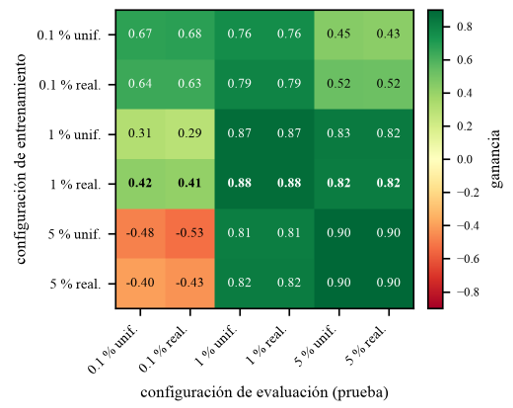
\includegraphics[width=\columnwidth]{figuras/fig4_matriz_entrenamiento_evaluacion.png}
  \caption{Ganancia en el conjunto de prueba de \emph{E. coli} de los 6 modelos finales (filas) en cada configuración de evaluación (columnas), promediada sobre las 5 semillas. En negrita, el modelo elegido con validación.}
  \Description{Mapa de calor de 6 por 6 con la ganancia en prueba de cada modelo final (filas) en cada configuración de evaluación (columnas).}
  \label{fig:matriz}
\end{figure}

\subsection{Intervalos de confianza y criterios de éxito}\label{sec:res-intervalos}

La Tabla~\ref{tab:bootstrap} presenta los intervalos de confianza del 95 \% obtenidos por bootstrap. En \emph{E. coli}, el límite inferior del intervalo de la ganancia del modelo ajustado fue mayor que 0 en todas las tasas y perfiles; el intervalo fue más amplio con el 0.1 \% (de 0.318 a 0.506 con errores realistas), ya que cada versión de esa configuración tiene solo cerca de 400 errores. Las diferencias de F1 de detección y de corrección frente al N-gramas fueron positivas y sus intervalos no incluyeron el 0 en ninguna configuración, tanto en \emph{E. coli} como en las arqueas. En las arqueas, la ganancia fue significativamente negativa con el 0.1 \% en ambos perfiles; su intervalo incluyó el 0 con el 1 \% realista (de −0.0004 a 0.009), y fue positiva, aunque pequeña, con el 1 \% uniforme y con el 5 \%.

\begin{table*}[t]
\caption{Estimados e intervalos de confianza del 95 \% por bootstrap}
\label{tab:bootstrap}
\small
\begin{tabular}{llllll}
\toprule
 & & \multicolumn{3}{c}{\textbf{Prueba E. coli}} & \textbf{H. volcanii} \\
\cmidrule(lr){3-5}\cmidrule(lr){6-6}
\textbf{Tasa} & \textbf{Perfil} & \textbf{Ganancia} & \textbf{Dif. F1 det.} & \textbf{Dif. F1 corr.} & \textbf{Ganancia} \\
\midrule
0.1 \% & uniforme & 0.425 {[}0.325, 0.511{]} & 0.767 {[}0.736, 0.796{]} & 0.764 {[}0.733, 0.792{]} & −0.596 {[}−0.666, −0.538{]} \\
 & realista & 0.413 {[}0.318, 0.506{]} & 0.766 {[}0.736, 0.796{]} & 0.762 {[}0.733, 0.792{]} & −0.593 {[}−0.658, −0.533{]} \\
\midrule
1 \% & uniforme & 0.877 {[}0.861, 0.891{]} & 0.939 {[}0.930, 0.946{]} & 0.934 {[}0.925, 0.941{]} & 0.008 {[}0.003, 0.012{]} \\
 & realista & 0.878 {[}0.863, 0.892{]} & 0.940 {[}0.932, 0.947{]} & 0.935 {[}0.927, 0.941{]} & 0.004 {[}−0.0004, 0.009{]} \\
\midrule
5 \% & uniforme & 0.819 {[}0.806, 0.831{]} & 0.905 {[}0.898, 0.912{]} & 0.895 {[}0.887, 0.903{]} & 0.037 {[}0.036, 0.039{]} \\
 & realista & 0.818 {[}0.804, 0.830{]} & 0.906 {[}0.898, 0.913{]} & 0.896 {[}0.887, 0.903{]} & 0.036 {[}0.034, 0.038{]} \\
\bottomrule
\end{tabular}

\vspace{2pt}\begin{minipage}{\textwidth}\footnotesize Ganancia del modelo ajustado y diferencia pareada «ajustado − N-gramas» en F1 de detección y de corrección (1000 réplicas, remuestreando genes completos con sus 5 versiones). Las diferencias de F1 en \emph{H. volcanii} también fueron positivas y excluyeron el 0 en todas las configuraciones (entre 0.11 y 0.16 en F1 de detección).\end{minipage}
\end{table*}

Con estos resultados, el modelo propuesto cumple los dos primeros criterios de éxito definidos en la sección~\ref{sec:criterios}: obtiene una ganancia mayor a 0 en todas las tasas y perfiles de \emph{E. coli}, y F1 de detección y de corrección mayores que los del N-gramas, con intervalos de la diferencia que no incluyen el 0. No cumple el tercero, ya que en las arqueas la ganancia fue negativa con el 0.1 \% de errores, tanto en la media como en todo su intervalo de confianza, y con el 1 \% realista el límite inferior de su intervalo fue menor que 0.

\section{Discusión}\label{sec:discusion}

En esta sección se interpretan los resultados de la sección anterior, relacionándolos con las decisiones de diseño descritas en las secciones~\ref{sec:simulacion} y~\ref{sec:metodologia} y con la analogía de la corrección ortográfica que guía el proyecto.

\subsection{El ajuste fino enseña al modelo cuándo corregir}\label{sec:disc-ajuste}

La comparación entre GENERanno sin ajuste y ajustado permite separar lo que el modelo ya sabía de lo que aprendió con el ajuste fino. Con detección perfecta, el modelo sin ajuste ya elige la base correcta en el 90.5 \% de los errores de \emph{E. coli}, muy por encima del N-gramas (47.2 \%) y del corrector por frecuencia (33.1 \%). Esto indica que el preentrenamiento con modelado de lenguaje enmascarado ya le da al modelo un conocimiento amplio de qué nucleótido encaja en cada contexto, y que este conocimiento depende de un contexto largo que el N-gramas, con un codón a cada lado, no alcanza a capturar. Lo que el modelo sin ajuste no sabe es cuándo cambiar una base: modifica cerca de 5 de cada 1,000 posiciones correctas sin importar cuántos errores tenga la secuencia, por lo que su ganancia es negativa cuando los errores son escasos. El ajuste fino redujo esta sobrecorrección cerca de 9 veces y, al mismo tiempo, subió la exactitud con oráculo del 90.5 \% al 98.5 \%; es decir, aportó sobre todo a la detección, que es justamente lo que diferencia la corrección de errores de la tarea de preentrenamiento.

Este comportamiento es el opuesto al que advierten Zhang et al.~\cite{zhang2020spelling} para BERT en la corrección ortográfica, donde el modelo tiende a copiar la entrada. Aquí, el modelo sin ajuste tiende a sobrecorregir, posiblemente porque su cabeza de lenguaje enmascarado predice la base más probable según el contexto incluso cuando la base observada es válida pero menos frecuente. El modelo ajustado tampoco se limitó a copiar la entrada pese al desbalance de clases: con w = 1 detectó el 93.7 \% de los errores con el 1 \%. De hecho, darle más peso a las posiciones con error empeoró la ganancia en validación (de 0.880 con w = 1 a 0.316 con w = 100), aunque el AUPRC se mantuvo prácticamente igual (entre 0.981 y 0.983); es decir, el modelo ordenaba los errores igual de bien, pero decidía peor cuándo cambiar una base, lo que es consistente con que un peso alto empuja al modelo a cambiar más posiciones, y la ganancia penaliza cada cambio indebido tanto como premia cada corrección. Por esto, para esta tarea y esta métrica, el riesgo de copiar la entrada que motivó la pérdida ponderada no se presentó, y el riesgo dominante fue el contrario.

\subsection{La tasa de error determina el valor de la ganancia}\label{sec:disc-tasa}

El resultado más relevante para el uso práctico del modelo es la dependencia de la ganancia con la tasa de error. La ganancia del modelo ajustado bajó de 0.878 con el 1 \% a 0.413 con el 0.1 \%, pero no porque el modelo sea peor encontrando o corrigiendo errores en esa tasa: detectó el 95.1 \% de los errores con el 0.1 \% y el 93.7 \% con el 1 \%, y, cuando se le indicó dónde estaban (oráculo), eligió la base correcta en el 98.6 \% y el 98.5 \% de los casos. La diferencia está en los cambios indebidos. El modelo cambia un número casi constante de posiciones correctas, unas 215 a 221 por versión del conjunto de prueba en ambas tasas (una por cada 1,860 a 1,930 posiciones correctas), y la ganancia resta esos cambios de los errores corregidos y divide entre el número de errores reales. Con el 1 \% hay 4,138 errores: el modelo corrige 3,855 e introduce 221, y la ganancia es (3,855 − 221) / 4,138 = 0.878. Con el 0.1 \% solo hay 403 errores: corrige 382, pero los 215 cambios indebidos pesan mucho más, y la ganancia baja a (382 − 215) / 403 ≈ 0.41. Por la misma razón, el 35.2 \% de los genes sin errores sale dañado con el 0.1 \%. Es importante resaltar este punto porque, según Stoler y Nekrutenko~\cite{stoler2021sequencing}, las tasas de error medianas de Illumina están entre 0.087 \% y 0.613 \%, es decir, más cerca del escenario más difícil para el modelo que del escenario con el que fue entrenado.

La matriz de la Fig.~\ref{fig:matriz} muestra que el modelo aprende, además de los patrones del ADN, una idea implícita de qué tan frecuentes son los errores, de forma similar al parámetro e del modelo de canal ruidoso: los modelos entrenados con el 5 \% cambian bases con más facilidad y obtienen ganancias negativas con el 0.1 \%, mientras que los entrenados con el 0.1 \% son más conservadores y dejan errores sin corregir cuando estos son abundantes. Así, si se conoce de antemano la tasa aproximada del secuenciador, conviene usar un modelo entrenado con una tasa cercana; con el 0.1 \%, por ejemplo, los modelos entrenados con esa tasa obtuvieron ganancias de 0.63 a 0.68, frente a 0.41 del modelo elegido. Si la tasa no se conoce, en cambio, conviene un modelo que funcione razonablemente bien en todas, y por eso se eligió el entrenado con el 1 \% realista, que tuvo la mayor ganancia promedio sobre las seis configuraciones de validación. Esta elección no fue casualidad del conjunto de validación: en prueba, con genes distintos, este modelo también tuvo la mayor ganancia promedio (0.705). Adicionalmente, el modelo podría ser más conservador sin necesidad de volver a entrenarlo. Con la regla actual, cambia una base siempre que considera que otra es más probable que la observada, sin exigir un nivel mínimo de seguridad. Una alternativa es usar el puntaje de sospecha con el que se calcula el AUPRC, 1 − P(base de entrada), y cambiar la base solo cuando este supere un umbral elegido en validación (por ejemplo, 0.9), de modo que el modelo corrija únicamente las posiciones de las que está muy seguro. Los resultados sugieren que este umbral sería útil: con el 0.1 \%, la regla actual opera con una precisión de detección de 0.640 y un recall de 0.951, mientras que el AUPRC, que promedia la precisión a lo largo de todos los niveles de recall, es de 0.919. Esto indica que, renunciando a una parte pequeña del recall, la precisión aumentaría mucho, y con tasas bajas eso reduciría los cambios indebidos, que son los que hacen caer la ganancia. Ajustar este umbral, o entrenar con una mezcla de tasas, no se exploró en este trabajo y es una alternativa directa para reducir los cambios indebidos.

\subsection{Las líneas base clásicas}\label{sec:disc-lineas-base}

El N-gramas terminó comportándose prácticamente como el corrector sin cambios. Su AUPRC, cerca del doble de la del azar, y su exactitud con oráculo del 47.2 \% (frente al 33.3 \% del azar) muestran que el contexto local sí da algunas pistas sobre la base correcta, pero no con la seguridad suficiente para compensar el costo de cambiar una base: las configuraciones que cambiaban más posiciones introducían más errores de los que corregían y obtenían ganancias negativas en validación, por lo que la selección favoreció la más conservadora. Como e = 0.1 está en el borde de los valores explorados, no se puede descartar que otros valores dieran una ganancia ligeramente distinta, aunque, por lo anterior, no se espera que esto cambie la conclusión. El corrector por frecuencia, por su parte, acertó prácticamente lo mismo que el azar (33.1 \% frente a 33.3 \%). Esto se debe a que elige la base de reemplazo según qué tan frecuente es cada base en el entrenamiento, y en E. coli las cuatro bases aparecen casi en la misma proporción (entre el 24.0 \% y el 27.4 \%, lo que corresponde a un contenido de GC cercano al 52 \%); por lo tanto, ponderar por frecuencia equivale casi a elegir al azar entre las tres bases restantes, y la frecuencia por sí sola no aporta información. Ambas líneas base confirman que el desempeño del modelo propuesto no se explica por regularidades simples de composición ni de contexto local, y respaldan el cumplimiento holgado del segundo criterio de éxito.

\subsection{Lo que el modelo aprendió del lenguaje del ADN}\label{sec:disc-lenguaje}

Los desgloses por categoría muestran que el modelo aprendió reglas propias del lenguaje de las secuencias codificantes. Los errores sin sentido, que crean un codón de parada en medio del gen, son los más fáciles de detectar (98.5 \%), lo que es coherente con que un codón de parada prematuro es muy anómalo dentro de una secuencia codificante. Los errores sinónimos, en cambio, son los más difíciles (85.6 \%): como no cambian el aminoácido, la secuencia con error sigue codificando la misma proteína, y el modelo solo puede reconocerlos por el uso de codones. Esta situación es análoga a los errores ortográficos que producen otra palabra válida (por ejemplo, «casa» por «caza»), que son los más difíciles para cualquier corrector, ya que no se pueden detectar mirando la palabra por sí sola. Lo mismo explica que la tercera posición del codón, donde se concentran los cambios sinónimos, sea la de menor recall y mayor sobrecorrección, y que las transiciones, que en la tercera posición suelen ser sinónimas, sean las más difíciles de detectar.

Los errores que introduce el modelo apuntan en la misma dirección: más de la mitad cae en la tercera posición, cerca de la mitad son sinónimos y la mayoría reemplaza un codón por uno más frecuente en el entrenamiento, como TTG→CTG o AAG→AAA. Es decir, el modelo tiende a «normalizar» codones válidos pero poco frecuentes hacia la forma más común, igual que un corrector ortográfico que cambia una palabra correcta pero rara por una más usual. Estos cambios indebidos rara vez cortan la proteína (solo el 0.36 \% crea un codón de parada), pero no son inocuos: el 52.0 \% cambia un aminoácido. Además, pueden ser un problema cuando la secuencia contiene variación natural. Dos cepas de una misma especie difieren en variantes reales de un solo nucleótido (SNPs), que no son errores de secuenciación, y el modelo se entrenó con una sola cepa de referencia. Como sus cambios indebidos se concentran en la tercera posición del codón y tienden a reemplazar codones poco frecuentes por otros más comunes, una variante real que use un codón poco frecuente sería «corregida» hacia la forma de la cepa de referencia, lo que borraría información biológica real; en aplicaciones como la tipificación de cepas o la detección de mutaciones de resistencia, esto equivaldría a reportar una secuencia que no existe. La escala del problema no es despreciable: el modelo introduce cerca de un cambio indebido cada dos genes (unos 215 por versión del conjunto de prueba, que tiene 433 genes) y, con el 0.1 \% de errores, dañó el 35.2 \% de los genes que no tenían ninguno. Como todas las secuencias de este trabajo provienen de una sola cepa, no fue posible medir cuántas variantes reales modificaría el modelo, lo que se retoma como trabajo futuro en la sección~\ref{sec:trabajo-futuro}. La preferencia por las transiciones (cambiar una base por otra del mismo tipo químico: una purina por otra, A↔G, o una pirimidina por otra, C↔T; ver sección~\ref{sec:res-categorias}) representa el 50 \% de los cambios indebidos, cuando al azar se esperaría un 33.3 \%, y se explica en parte por el código genético. En los aminoácidos codificados por dos codones, como el ácido aspártico (GAT y GAC) o la lisina (AAA y AAG), los dos codones difieren solo en la tercera base y por una transición, de modo que el único cambio sinónimo posible es una transición. Para medir este efecto, se tomaron todos los cambios de una sola base que se pueden hacer sobre los codones de los genes de entrenamiento de E. coli, ponderados por qué tan frecuente es cada codón, y se separaron en dos grupos: los sinónimos, que mantienen el aminoácido, y los que lo cambian. Entre los sinónimos, el 49.1 \% son transiciones; entre los que cambian el aminoácido, solo el 28.5 \%. Es decir, un cambio sinónimo es mucho más probable que sea una transición que un cambio que altera la proteína. Como el 48 \% de los cambios indebidos del modelo son sinónimos y el 52 \% no, si el modelo eligiera al azar dentro de cada grupo se esperaría que cerca del 38 \% fueran transiciones (0.48 × 49.1 \% + 0.52 × 28.5 \%). El 50 \% observado supera este valor, y 9 de los 10 cambios indebidos más repetidos fueron transiciones, por lo que el modelo tiene una preferencia adicional por ellas. Una posible explicación es que en la variación natural del ADN, con la que se preentrenó el modelo, las transiciones son más frecuentes que las transversiones~\cite{wakeley1996excess}, aunque esto no se verificó en este trabajo. Este patrón es propio de E. coli: en las arqueas, solo el 33.6 \% de los cambios indebidos del modelo ajustado fueron transiciones, prácticamente lo esperado al azar, y apenas el 7.6 \% fueron sinónimos, lo que coincide con que el modelo aprendió el uso de codones de E. coli y no lo reconoce en otro organismo.

En los codones de inicio y de parada, que tienen muy pocas formas válidas, el modelo ajustado casi no hizo cambios indebidos y aumentó el porcentaje de genes con estos codones correctos. El modelo sin ajuste, en cambio, alteró más de la tercera parte de los codones de parada correctos. Al revisar este comportamiento en los genes de arqueas, donde ocurrió lo mismo, el efecto resultó ser propio del codón de parada: el modelo sin ajuste cambió el 33.3 \% de las bases correctas de ese codón, frente al 2.5 \% de todas las posiciones correctas del gen. El codón de inicio, que tampoco tiene contexto a un lado, casi no se modificó (0.3 \% de sus bases correctas). Esto indica que el modelo sin ajuste no reconoce bien el codón de parada cuando está al final de la secuencia, aunque en este trabajo no se pudo determinar la causa. El ajuste fino eliminó este comportamiento (en las arqueas, solo el 0.09 \% de las bases correctas del codón de parada cambiaron, y el 0.27 \% de los genes quedó con ese codón dañado), lo que es un ejemplo concreto de cómo el ajuste adapta el modelo al formato de entrada de la tarea, en el que cada secuencia termina justo en su codón de parada.

\subsection{Generalización fuera de dominio}\label{sec:disc-dominio}

El modelo no cumplió el criterio de éxito en las arqueas, y el análisis muestra que la falla está en la detección y no en el conocimiento de qué base corresponde: con oráculo, el modelo ajustado acertó en el 67.4 \% de los errores, el doble que el azar, pero detectó menos del 10 \% de ellos. Esto sugiere que el modelo conserva parte del conocimiento general del ADN, pero que su criterio para decidir que una base es un error quedó calibrado para \emph{E. coli}: ante secuencias poco familiares tiende a confiar en la base observada y deja la mayoría de los errores sin cambiar, mientras que buena parte de los pocos cambios que hace son indebidos (precisión de detección de 0.124 con el 0.1 \%). Una causa probable es la diferencia de composición: \emph{H. volcanii} tiene un contenido de GC de 66.6 \%, y de 86.1 \% en la tercera posición de los codones, un rango que no aparece en el entrenamiento; además, dentro de \emph{E. coli} el modelo ya mostró que su ganancia baja en los genes de composición atípica (0.499 en los genes con menos del 40 \% de GC). Esto es comparable a usar un corrector ortográfico entrenado en un idioma sobre textos de otro idioma cercano: reconoce parte del vocabulario, pero no distingue con seguridad qué es un error.

El modelo sin ajuste también tuvo un desempeño mucho menor en las arqueas (62.4 \% con oráculo, frente a 90.5 \% en \emph{E. coli}), lo que es coherente con que, según sus autores, GENERanno no se preentrenó con arqueas. Esto refuerza la limitación mencionada en la sección~\ref{sec:limitaciones}: parte del buen desempeño en \emph{E. coli} probablemente proviene de lo aprendido en el preentrenamiento, que pudo incluir genomas de este organismo, y la prueba con arqueas muestra que ese desempeño no se transfiere directamente a otros dominios. Aun así, el modelo ajustado obtuvo una ganancia mucho mayor que la del modelo sin ajuste en todas las tasas, y con el 5 \% su ganancia fue positiva con un intervalo que no incluye el 0, aunque demasiado pequeña (0.036) para que el modelo sea útil en este organismo sin entrenarlo también con genes de arqueas o de organismos con una composición parecida.

\subsection{Validez de los resultados}\label{sec:disc-validez}

Varios elementos del protocolo respaldan la solidez de estos resultados. La partición se verificó exactamente antes de evaluar, por lo que ningún gen de prueba ni de su grupo de similitud se usó para entrenar o elegir los modelos. La desviación estándar entre las 5 semillas y los intervalos por bootstrap fueron pequeños con el 1 \% y el 5 \%, por lo que las diferencias entre modelos no dependen de los errores sorteados ni de los genes particulares del conjunto de prueba, y la matriz de prueba reprodujo la de validación, lo que indica que la elección del modelo no se sobreajustó al conjunto de validación. Por otro lado, los resultados con el 0.1 \% son menos precisos (el intervalo de la ganancia tiene un ancho cercano a 0.19), ya que se basan en cerca de 400 errores por versión. En 4 de los 11 entrenamientos la mejor época fue la última, por lo que es posible que más épocas mejoraran ligeramente los modelos, aunque en esos casos la ganancia en validación ya aumentaba menos de 0.003 entre las dos últimas épocas.

Por último, el perfil de error casi no cambió los resultados de ningún modelo. Esto puede deberse a que el perfil realista acentúa los sesgos de Illumina de forma moderada y a que, al estar normalizado, introduce en promedio la misma cantidad de errores que el uniforme (sección~\ref{sec:simulacion}). Por esto, aunque el modelo resultó robusto entre los dos perfiles simulados, no se puede concluir que lo sea frente a perfiles reales con sesgos más fuertes.

\subsection{Limitaciones}\label{sec:limitaciones}

Solo se consideraron sustituciones; las inserciones y deleciones, que dominan en tecnologías como PacBio, no están contempladas dentro de este trabajo. Los errores se simularon sobre secuencias codificantes y no sobre lecturas reales, por lo que los resultados no son comparables directamente con los correctores, que operan sobre lecturas con cobertura. En adición, el perfil realista es una simplificación donde sus parámetros son lecturas de 150 nucleótidos, pendiente de 3, factor de 3 tras homopolímeros y 50 \% de repetición de la base anterior elegidos para acentuar moderadamente los sesgos de~\cite{stoler2021sequencing} y no se estimaron con datos reales, y no se simularon otros sesgos como los trímeros sobrerrepresentados.

GENERanno pudo haber visto genomas de \emph{E. coli} durante el preentrenamiento, por lo que parte del desempeño en este organismo podría estarse viendo influenciado por esto; y aunque la prueba que efectuamos con (\emph{H. volcanii}) puede ayudar a mitigar este riesgo no permite generalizar a todo el dominio. Por restricciones computacionales el lote fue de 4 genes, donde solo evaluamos secuencias codificantes, sin regiones intergénicas, así mismo no podemos diferenciar con claridad un error de secuenciación de una variación natural.

\subsection{Consideraciones éticas}\label{sec:etica}

Las consideraciones más importantes parten del uso de datos, en nuestro caso todos los datos de genomas de referencia son datos públicos no humanos, por lo que no requieren consentimiento informado ni aprobación de un comité de ética, así mismo el NCBI no impone restricciones al uso de estos datos, aunque sí existe una advertencia donde los depositantes originales pueden reclamar derechos sobre parte de la información.

El modelo desarrollado en el presente trabajo tiende a ``normalizar'' codones válidos pero poco frecuentes hacia los más comunes. Esto en un contexto clínico o de investigación clínica podría llevar a borrar variantes naturales reales o algún tipo de mutación relevante. Por eso el modelo no debe usarse con el fin de hacer corrección de datos con fines diagnósticos. Además, el modelo falló fuera de su dominio de entrenamiento (ganancia negativa con el 0.1 \% en arqueas), de modo que no debería aplicarse a organismos distintos a \emph{E. coli} sin evaluarlo primero en ellos.

Declaramos las decisiones de diseño que pueden afectar los resultados: los parámetros del perfil de error realista fueron elegidos por nosotros y no estimados con datos reales, la partición se hizo por gen, los errores de prueba se fijaron con semillas conocidas y se reportan intervalos de confianza, y también reportamos los criterios de éxito que no se cumplieron.

\section{Conclusiones y trabajo futuro}\label{sec:conclusiones}

Este trabajo propone ajustar el modelo de GENERanno con LoRA y una cabeza de clasificación para la tarea de corrección de errores de sustitución en secuencias codificantes completas de ADN. Para esto se realizó un entrenamiento y validación sobre secuencias codificantes de E. coli y se evaluó sobre este mismo genoma y sobre un genoma fuera del dominio (H. volcanii).

Este trabajo propone una analogía donde las secuencias de ADN corresponden a oraciones de texto, los codones a palabras y los nucleótidos a letras. De los experimentos se puede concluir que el modelo tuvo cierto nivel de aprendizaje del lenguaje del ADN. Se observó que entendió cuáles eran los codones de inicio y de fin, ya que casi no introdujo errores en ellos y corrigió la mayoría de los errores encontrados en estos codones, aunque los detectó menos que los del interior del gen. También detectó casi siempre cuando se formaba erróneamente un codón de fin de manera prematura. Adicionalmente, se observó que al modelo se le dificultó más detectar errores en los cuales el codón se transformaba en un sinónimo, ya que el codón resultante sigue siendo válido y codifica el mismo aminoácido. Esto es algo que se observa en correctores ortográficos cuando un error produce una palabra válida. Además, cuando el modelo introdujo errores, cerca de la mitad de los cambios fueron por sinónimos y la mayoría hacia codones más frecuentes, lo que sugiere un comportamiento de normalización de las secuencias, comportamiento que se puede ver en correctores ortográficos que corrigen por la secuencia más probable.

Al evaluar el modelo propuesto, se comparó con una serie de líneas base de referencia: el corrector sin cambios, el corrector por frecuencia, el modelo de n-gramas y el mismo GENERanno sin ajustar. El modelo propuesto obtuvo la mayor ganancia en todas las tasas en el conjunto de E. coli, logrando ganancias superiores a 0.8 para las tasas de 1 \% y 5 \% y cercanas a 0.4 para el 0.1 \%, superando al n-grama por entre 0.4 y 0.9 y al modelo sin ajustar por entre 0.38 y 0.65 con el 1 \% y el 5 \%. Esto se explica por la combinación del vasto preentrenamiento de GENERanno, que le da el conocimiento de qué base encaja en cada contexto, y el ajuste fino, que le enseñó cuándo corregir. No obstante, el modelo quedó muy ajustado a las distribuciones de E. coli, posiblemente por la diferencia en el contenido de GC de las arqueas y porque el preentrenamiento pudo incluir genomas de E. coli. Por esto, en el conjunto de arqueas, el rendimiento fue muy bajo y se comportó de forma muy conservadora al no lograr detectar los errores. Aun así, superó al modelo sin ajustar en todas las tasas, aunque con el 0.1 \% quedó por debajo del corrector sin cambios. Con detección perfecta, eligió la base correcta en el 67.4 \% de los errores, el doble que el corrector por frecuencia.

Es muy importante resaltar el hecho de que el modelo mejoró ampliamente la detección de errores frente al modelo sin ajustar al evaluar sobre E. coli y redujo cerca de 9 veces la sobrecorrección. Por otra parte, el modelo de n-gramas casi no hizo cambios, ya que sus probabilidades rara vez superaron el costo de cambiar una base que impone el parámetro e.

Otra observación es que, al entrenar los mismos modelos con varias tasas de error propuestas, estos se ajustan a la frecuencia de error observada en entrenamiento y, en consecuencia, tienen un rendimiento degradado sobre otras tasas. Por esto mismo, se propone usar un modelo entrenado con una tasa cercana a la del secuenciador cuando esta se conoce, y uno entrenado con una tasa intermedia, como el 1 \%, cuando no se conoce. Esto es especialmente importante porque las tasas medianas de Illumina están entre 0.087 \% y 0.613 \%, donde la ganancia del modelo elegido es menor: 0.41 con el 0.1 \%.

Otro hallazgo del proyecto es que dar más peso a los errores en el cálculo de la pérdida para contrarrestar el desbalance de las clases empeoró la ganancia, probablemente porque el modelo cambia más posiciones correctas; por esto, con los pesos explorados y la ganancia como métrica, la ponderación de la pérdida no resultó útil en este caso.

Respecto a los criterios de éxito definidos, se lograron 2 de 3. Se logró conseguir una ganancia mayor a 0 en todas las tasas y perfiles de E. coli, es decir, se hicieron más correcciones que daños a las secuencias. Además, la ganancia fue significativamente mayor que el punto de balance (ganancia 0), siendo superior a 0.8 para las tasas de error de 1 \% y 5 \% y cercana a 0.4 para el conjunto de 0.1 \%. También se superó a los n-gramas en F1 de detección y corrección con un intervalo de confianza de la diferencia que no incluye el 0, siendo el valor más bajo del intervalo entre todas las tasas 0.73. Finalmente, no se logró obtener una ganancia mayor a 0 en todas las tasas de los conjuntos de prueba con arqueas: con el 0.1 \% fue negativa, por las razones ya explicadas.

\subsection{Trabajo futuro}\label{sec:trabajo-futuro}

Una primera línea es validar con lecturas reales de baja cobertura y estimar el perfil de error a partir de datos reales en lugar de fijarlo a mano. Otra es extender el modelo a inserciones y deleciones, lo que exigirá una pérdida o un esquema de alineamiento como el de~\cite{baid2021deepconsensus}. También sería valioso entrenar el modelo para distinguir errores de variantes reales (SNPs) y medir los falsos positivos sobre variación natural, ya que hoy el modelo podría «corregir» codones poco frecuentes pero válidos. .

Como los resultados muestran que la mayor parte de lo que el modelo deja sin corregir se pierde en la detección y no en la elección de la base, una línea prometedora es separar ambas tareas con un modelo dedicado a detectar errores. Soft-Masked BERT~\cite{zhang2020spelling} lo hace con una red de detección (Bi-GRU) que estima la probabilidad de error de cada posición y la usa para enmascarar suavemente la entrada de la red de corrección. Una arquitectura similar, o simplemente un umbral sobre el puntaje de sospecha del modelo actual, podría reducir los cambios indebidos y mejorar la ganancia con tasas de error bajas.

Otra línea es combinar los métodos tradicionales con nuestra técnica y evaluar si hay mejora. Por ejemplo, el modelo de n-gramas podría aportar una segunda señal de detección que se combine con las probabilidades del modelo ajustado, o los correctores basados en k-mers~\cite{mitchell2020benchmarking} podrían aplicarse cuando haya cobertura suficiente y reservar el modelo para las lecturas de baja cobertura. Por último, el parámetro e del modelo de n-gramas quedó en el borde inferior de los valores explorados (0.1), por lo que sería útil ampliar su rango con valores menores, para confirmar que la conclusión sobre esta línea base no cambia. Quedan también pendientes la ablación de la tokenización frente a DNABERT-2 (BPE), entrenar con una mezcla de tasas de error y evaluar más organismos, incluidas otras arqueas y eucariotas.

\bibliographystyle{ACM-Reference-Format}
\bibliography{referencias}

\end{document}
